\documentclass{sigplanconf}

\usepackage[usenames]{color}
\definecolor{citationcolour}{rgb}{0,0.4,0.2}
\definecolor{linkcolour}{rgb}{0,0,0.8}
\usepackage{hyperref}
\hypersetup{colorlinks=true,
            urlcolor=linkcolour,
            linkcolor=linkcolour,
            citecolor=citationcolour,
            pdftitle=Abstraction and Invariance for Algebraically Indexed Types,
            pdfauthor={Robert Atkey, Patricia Johann, Andrew Kennedy},
            pdfkeywords={}}  
\def\sectionautorefname{Section}
\def\subsectionautorefname{Section}
\def\subsubsectionautorefname{Section}

\title{Abstraction and Invariance for Algebraically Indexed Types}

\authorinfo{Robert Atkey\and Patricia Johann}
           {University of Strathclyde}
           {$\{$Robert.Atkey,Patricia.Johann$\}$@strath.ac.uk}

\authorinfo{Andrew Kennedy}
           {Microsoft Research Cambridge}
           {akenn@microsoft.com}

\usepackage{mathpartir}
\usepackage{amsmath}
\usepackage{amssymb}
\usepackage{amsthm}
\usepackage{stmaryrd}
\usepackage{pgf}
\usepackage{tikz}
\usepgflibrary{shapes.geometric}
\usepgflibrary{shapes.misc}
\usepgflibrary{shapes.multipart}
\usetikzlibrary{shapes.geometric}
\usetikzlibrary{shapes.misc}
\usetikzlibrary{shapes.multipart}

\newcommand{\todo}[1]{[\textbf{TODO}: #1]}

\newcommand{\abs}[1]{\lvert #1 \rvert}

\newcommand{\GL}[1]{\mathrm{GL}_#1}
\newcommand{\SynGL}[1]{\mathsf{GL}_#1}
\newcommand{\SE}[1]{\mathsf{SE}_#1}
\newcommand{\SynSE}[1]{\mathsf{SE}_#1}
\newcommand{\Orth}[1]{\mathrm{O}_#1}
\newcommand{\SynOrth}[1]{\mathsf{O}_#1}
\newcommand{\Transl}[1]{\mathrm{T}_#1}
\newcommand{\SynTransl}[1]{\mathsf{T}_#1}
\newcommand{\Scal}{\mathrm{Scal}}
\newcommand{\SynScal}{\mathsf{Scal}}

\newcommand{\sepbar}{\mathrel|}

\newcommand{\Rel}{\mathrm{Rel}}
\newcommand{\relArrow}{\mathrel{\widehat\to}}
\newcommand{\relTimes}{\mathrel{\widehat\times}}
\newcommand{\relSum}{\mathrel{\widehat+}}
\newcommand{\Eq}{\mathrm{Eq}}

\newcommand{\setOfIntegers}{\mathbb{Z}}
\newcommand{\setOfBooleans}{\{\tmTT, \tmFF\}}

\newcommand{\id}{\mathrm{id}}

\newcommand{\SortSet}{\mathit{Sort}}
\newcommand{\IndexOpSet}{\mathit{IndexOp}}
\newcommand{\PrimTypeSet}{\mathit{PrimType}}
\newcommand{\IndexAxiomSet}{\mathit{IndexAx}}

\newcommand{\indexOp}[1]{\textup{\texttt{#1}}}
\newcommand{\idxTms}[2]{\mathrm{IdxTm}(#1 \vdash #2)}
\newcommand{\idxTmAS}[1]{\mathrm{IdxTm}(#1)}

\newcommand{\tyInt}{\texttt{int}}
\newcommand{\tyBool}{\texttt{bool}}
\newcommand{\tyUnit}{\texttt{unit}}
\newcommand{\tyReal}{\texttt{real}}
\newcommand{\tyPrim}[2]{\textup{\texttt{#1}}\langle #2 \rangle}
\newcommand{\tyPrimNm}[1]{\textup{\texttt{#1}}}
\newcommand{\primTyArity}{\mathrm{tyArity}}
\newcommand{\indexOpArity}{\mathrm{opArity}}

\newcommand{\tyArr}{\to}
\newcommand{\tyProduct}{\times}
\newcommand{\tyX}[1]{\texttt{X}\langle #1 \rangle}
\newcommand{\isType}{\textup{\textsf{ type}}}
\newcommand{\isCtxt}{\textup{\textsf{ ctxt}}}
\newcommand{\Ty}{\textsf{Ty}}
\newcommand{\ty}{\textsf{ty}}

\newcommand{\tmTT}{\texttt{tt}}
\newcommand{\tmFF}{\texttt{ff}}

\newcommand{\relEnv}[1]{\mathcal{#1}}
\newcommand{\tySem}[1]{\left\lfloor #1 \right\rfloor}
\newcommand{\ctxtSem}[1]{\left\lfloor #1 \right\rfloor}
\newcommand{\tmSem}[1]{\left\lfloor{#1}\right\rfloor}
\newcommand{\tyPrimSem}[1]{\left\lfloor #1 \right\rfloor}
\newcommand{\rsem}[1]{\llbracket #1 \rrbracket}
\newcommand{\extends}[2]{\mathsf{ext}(#1,#2)}

\newtheorem{lemma}{Lemma}
\newtheorem{theorem}{Theorem}
\newtheorem{definition}{Definition}
\newcommand{\lemref}[1]{\hyperref[#1]{Lemma~\ref*{#1}}}
\newcommand{\thmref}[1]{\hyperref[#1]{Theorem~\ref*{#1}}}
\newcommand{\defref}[1]{\hyperref[#1]{Definition~\ref*{#1}}}
\newcommand{\propref}[1]{\hyperref[#1]{Proposition~\ref*{#1}}}
\newcommand{\corref}[1]{\hyperref[#1]{Corollary~\ref*{#1}}}
\newcommand{\conref}[1]{\hyperref[#1]{Conjecture~\ref*{#1}}}
\newcommand{\exref}[1]{\hyperref[#1]{Example~\ref*{#1}}}
\newcommand{\statementref}[1]{\hyperref[#1]{Statement~\ref*{#1}}}

\newcommand{\sem}[1]{\llbracket #1 \rrbracket}
\newcommand{\isDefinedAs}{\stackrel{\mathit{def}}=}

\newcommand{\Geom}{\mathit{2D}}

\newtheoremstyle{examplestyle}
  {\topsep}  % space above
  {\topsep}  % space below
  {\normalfont}% name of font to use in the body of the theorem
  {0em}% measure of space to indent
  {\bfseries}% name of head font
  {.}% punctuation between head and body
  {5pt plus 1pt minus 1pt}% space after theorem head; " " = normal interword space
  {}% Manually specify head
\theoremstyle{examplestyle}
\newtheorem{example}{Example}
\newtheorem*{example*}{Example}

\newtheoremstyle{restatementstyle}
  {\topsep}  % space above
  {\topsep}  % space below
  {\itshape}% name of font to use in the body of the theorem
  {0em}% measure of space to indent
  {\bfseries}% name of head font
  {.}% punctuation between head and body
  {5pt plus 1pt minus 1pt}% space after theorem head; " " = normal interword space
  {\thmname{#1} \thmnote{(Restatement of #3)}}% Manually specify head
\theoremstyle{restatementstyle}
\newtheorem{restateLemma}{Lemma}
\newtheorem{restateTheorem}{Theorem}

\newcommand{\fixme}[1]{\textbf{FIXME: #1}}

\begin{document}

\conferenceinfo{POPL'13,} {January 23--25, 2013, Rome, Italy.}
\CopyrightYear{2013}
\copyrightdata{978-1-4503-1832-7/13/01}

\maketitle

\begin{abstract}
  Reynolds' relational parametricity provides a powerful way to reason
  about programs in terms of invariance under changes of data
  representation. A dazzling array of applications of Reynolds' theory
  exists, exploiting invariance to yield ``free theorems'',
  non-inhabitation results, and encodings of algebraic datatypes.
  Outside computer science, invariance is a common theme running
  through many areas of mathematics and physics. For example, the area of
  a triangle is unaltered by rotation or flipping. If we scale a
  triangle, then we scale its area, maintaining an invariant
  relationship between the two. The transformations under which
  properties are invariant are often organised into groups, with the
  algebraic structure reflecting the composability and invertibility
  of transformations.

  In this paper, we investigate programming languages whose types are
  indexed by algebraic structures such as groups of geometric
  transformations. Other examples include types indexed by
  principals--for information flow security--and types indexed by
  distances--for analysis of analytic uniform continuity
  properties. Following Reynolds, we prove a general Abstraction
  Theorem that covers all these instances. Consequences of our
  Abstraction Theorem include free theorems expressing invariance
  properties of programs, type isomorphisms based on invariance
  properties, and non-definability results indicating when certain
  algebraically indexed types are uninhabited or only inhabited by
  trivial programs.  We have fully formalised our framework and most
  examples in Coq.
\end{abstract}

\category{D.1.1}{Programming techniques}{Applicative (functional)
  programming} \category{D.2.4}{Software Engineering}{Software/Program
  Verification} \category{D.3.3}{Programming Languages}{Language
  Constructs and Features---Data types and structures}

\terms
  Languages, Theory, Types

\keywords parametricity, units of measure, dimensional analysis,
invariance, computational geometry, information flow, metric types, uniform continuity

%%%%%%%%%%% Springe nach section-introduction.tex
%%%---------- open: section-introduction.tex
\section{Introduction}
\label{sec:introduction}
The best way we know of describing the semantics of parametric
polymorphism is \emph{relational parametricity}, whose central result
is Reynolds' Abstraction Theorem~\cite{reynolds83types}. Its striking
consequences include the well-known ``free theorems'' for polymorphic
types~\cite{wadler89theorems}, non-inhabitation results, and precise
correspondences between System F encodings and algebraic
datatypes~\cite{PittsAM:parpoe}, abstract data types, and, most
recently, higher-order encodings of binder
syntax~\cite{syntaxforfree}.

Relational parametricity is in essence a principle of
\emph{invariance}: the behaviour of polymorphic code is invariant
under changes of data representation. For example, the type
$\forall\alpha.\tyPrim{list}\alpha\to\tyPrim{list}\alpha$
tells us that any transformation applied to elements of
the input list will be reflected by the same transformation applied
to elements of the result. 
Invariance results also abound in
mathematics and physics. The area of a triangle is invariant with
respect to isometries of the Euclidean plane; the determinant of a
matrix is invariant under changes of basis; and Newton's laws are the
same in all inertial frames. Typically, the 
transformations under which invariants are preserved have interesting structure: 
for example, translations in
the Euclidean plane form an abelian group.

Inspired by this connection, we study type systems that
capture rich invariants in types indexed by attributes with
algebraic structure.  For example, in computational geometry, points
in the plane can be indexed by attributes representing affine
transformations; in information-flow security, computations can be
indexed by principals; in differential privacy, types can be indexed
by `distance'. Types that are polymorphic over such indices induce
invariance properties and abstraction barriers beyond those introduced
by their unindexed versions, as we shall illustrate.  This generalises
previous work by the third author on types parameterized by
units of measure, whose invariance properties relate to changes of
units, or \emph{scaling}~\cite{kennedy97relational}.


\paragraph{Invariance}
To illustrate type-induced invariance properties, consider
two-dimensional geometry. 
In a conventional type system, a function $\mathrm{areaTri}$ that computes the area of a triangle
might be assigned the type:
$\tyPrimNm{vec}\times\tyPrimNm{vec}\times\tyPrimNm{vec}\tyArr\tyReal$.
But in our proposed system we can assign it the following more expressive polymorphic
type:
\[
\mathrm{areaTri} : \forall t\mathord:\SynTransl{2}.
  \tyPrim{vec}{t} \times \tyPrim{vec}{t} \times \tyPrim{vec}{t} \to \tyReal \\
\]
This type expresses the fact that if each of the arguments to $\mathrm{areaTri}$
is translated by the same vector, then the result remains the same,
that is, it is \emph{invariant} under translation. Formally, for any 
vector $\vec t$,
\[
\mathrm{areaTri}\;(\vec{t} + \vec{v_1}, \vec{t} + \vec{v_2}, \vec{t} + \vec{v_3}) = 
\mathrm{areaTri}\;(\vec{v_1}, \vec{v_2}, \vec{v_3})
\]

Transformations typically \emph{compose} in various
ways, and the compositions satisfy algebraic laws. For example, 
we can assign a function that computes the area of a circle given its
radius the following polymorphic type:
\[
\mathrm{areaCircle} : \forall s\mathord:\SynGL{1}.\tyPrim{real}{s}\to
\tyPrim{real}{s\cdot s}
\]
This captures the fact that the area of a circle varies as the square
of its radius, i.e., $\mathrm{areaCircle}(k r) = k^2\cdot
\mathrm{areaCircle}(r)$ for any $k\neq 0$ (the `sorts' $\SynTransl{2}$ and
$\SynGL{1}$ will be explained later).  Here, $s$ 
can be interpreted as the \emph{units of measure} of the argument to
$\mathrm{areaCircle}$, and `$\cdot$' composes units using the
product. We can also add an inverse operation and identity unit of
measure $1$, and then impose the algebraic laws of abelian
groups. This permits identification of, for example,
$\tyPrim{real}{s\cdot s^{-1}}$ with the type
$\tyPrim{real}{1}$ of dimensionless constants.

\paragraph{Abstraction}
In his original paper on parametricity, Reynolds asserted that
\emph{type structure is a syntactic discipline for enforcing levels of
  abstraction}.  We see something analogous here: if all primitive
operations are given types that reflect their behaviour under
translation, then there is no way to `break' this property. For
example, there is no way that $\mathrm{areaTri}$ can depend on the
actual coordinates of its inputs. Furthermore, the distinction between
points and vectors that is often enforced through abstract data
types~\cite{CGAL} is captured here by indices instead. For example,
the operation that takes two points and computes their vector
difference can be assigned the type
$\forall t\mathord:\SynTransl{2}.\tyPrim{vec}t\times\tyPrim{vec}t\to\tyPrim{vec}0$,
reflecting the invariance of the result (a pure vector) under
translations of the point arguments. As a result through types alone
we can, in essence, derive so-called \emph{coordinate-free}
geometry~\cite{CFGADT}.

The invariance properties discussed above can be seen as ``free
theorems''~\cite{wadler89theorems}, but the abstraction afforded by
polymorphic indexed types can also induce interesting type
\emph{isomorphisms}.  The type of $\mathrm{areaCircle}$ above is in
fact isomorphic to $\tyPrim{real}{1}$. A moment's thought reveals why:
what possible unary functions can be constructed whose outputs scale
as the square of the scaling of their inputs?  Answer: just those
functions of the form~$\lambda x. k x^2$ for some constant~$k$.  In
this case, of course, we expect that~$k = \pi$.

\paragraph{Relational parametricity}
To derive such invariance and abstraction properties of types, we
adopt the techniques of relational parametricity. Over an underlying
index-erasure semantics we construct binary relations parameterised by
an environment $\rho$ that describes how values of primitive type are
related according to their indices.  For example, values $v$ and $w$
of type $\tyPrim{real}s$ are related when $v$ ``scales to'' $w$
according to an interpretation of $s$ (i.e., $w=\rho(s)\cdot
v$).  Values of polymorphic type are related exactly when they are
related for all possible interpretations of the quantified
variable. For example, values $v$ and $w$ of type
$\forall t\mathord:\SynTransl{2}.\tyPrim{vec} t\to
\tyPrim{vec} t$ are related when they are related at type
$\tyPrim{vec} t\to\tyPrim{vec}t$ for all translations
$\vec t\in\Transl{2}$ associated with $t$.

As it happens, the relational interpretations given above are
functional, relating one value uniquely to another. Other applications
make use of primitive relations that are not simple functions.
For example, in a type system in which the index in
$\tyPrim{real}s$ is interpreted not as a unit of measure, but as
a measure of \emph{closeness}, two values $x$ and $y$ of this type are
related if $|x-y| < \rho(s)$ for a positive real number
$\rho(s)$.  Rather beautifully, the standard notion of uniform
continuity can then be expressed as %a type:
%\begin{displaymath}
 $ \forall \epsilon \mathord: \mathsf{R}^{>0}.\ \exists \delta\mathord: \mathsf{R}^{>0}.\ \tyPrim{real}{\delta} \to \tyPrim{real}{\epsilon}$.
%\end{displaymath}

\paragraph{Motivations}
Our motivations for studying algebraically indexed types are
threefold. First, we believe that, as with
units of measure~\cite{fsharp}, practical programming language
extensions will follow. For example, in computational geometry and
graphics, attributes on points, vectors, and other geometric types
could be used to prevent the mixing of different coordinate systems,
or `frames'. Second, type-based static analyses can be based on
indexed types, for example, in effect systems~\cite{benton06reading},
and, more speculatively, in continuity
analysis~\cite{chaudhuri10continuity}.  Finally, we believe that
expressing algebraic invariants through types has the potential to
offer slick proof techniques for mechanized
mathematics. Harrison has applied the
invariance properties of geometric primitives to create elegant proofs
in geometry, based on `without loss of
generality' principles~\cite{harrison09without}. The invariance properties are expressed 
and propagated using ad-hoc tactics; our types offer a more principled
means of achieving the same end, and the `wlog' principle itself
is expressed through type isomorphisms.

We follow the mantra \emph{semantics first, syntax later} in studying
types with algebraic structure. We have not yet built a practical
programming language that supports algebraically indexed types; nor
have we designed type checking, type inference, or static analysis
algorithms.  But when we do so, the semantics will guide us. The fact
that zero is polymorphic in units of measure (it can be given type $\forall
u.\tyPrim{real}u$) whereas other constants are dimensionless (having
type $\tyPrim{real}1$) is justified by the invariance properties
induced by the types: zero is invariant under scaling, other constants
are not. For less trivial constants and operations, the appropriate types are
not so apparent, as we shall see, but invariance properties expressed by
the semantics guide us in assigning appropriate types. Semantics does not lie!


% Possible angles of attack:
% \begin{itemize}
% \item Parametric polymorphic types allow us to prevent
%   over-specification of the behaviour of programs. For instance, the
%   type $\forall \alpha. [\alpha] \to [\alpha]$ is a generalisation of
%   the types $[\mathsf{int}] \to [\mathsf{int}]$ and $[\mathsf{char}]
%   \to [\mathsf{char}]$. Either of the latter two types over-specify
%   the behaviour of the function.
% \item There are other cases of programs that are over-specified. The
%   leading example we just below is of geometric programs that
%   manipulate coordinate data. Often, programs that manipulate
%   coordinate data are insensitive to geometric transformations. For
%   example, a program that computes the area of a triangle described by
%   three points is insensitive to translations or rotations applied to
%   all three points.
% \item 
% \end{itemize}

% There are three main points to get across:
% \begin{enumerate}
% \item Why algebraically indexed types?
% \item Why relational parametricity?
% \item Why study them together?
% \end{enumerate}

\subsection{Contributions}
\label{sec:contributions}

\begin{figure}
  \centering
  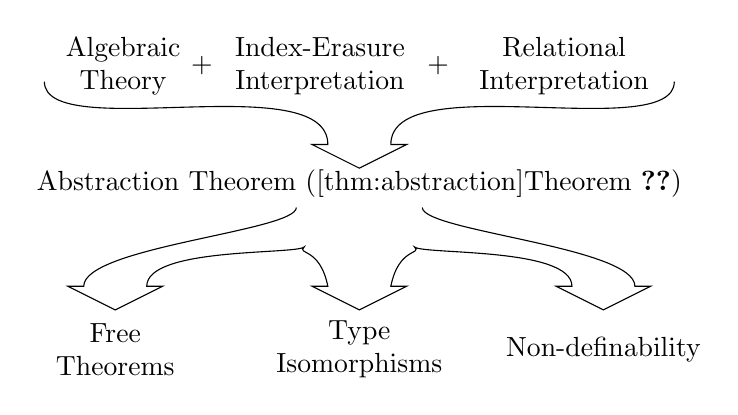
\begin{tikzpicture}
  \node at (-3,0.8) [rectangle,style={align=center}] {Algebraic \\ Theory};
  \node at (-2,0.8) {$+$};
  \node at (-0.5,0.8) [rectangle,style={align=center}] {Index-Erasure \\ Interpretation};
  \node at (1,0.8) {$+$};
  \node at (2.6,0.8) [rectangle,style={align=center}] {Relational \\ Interpretation};
  
  \draw plot (-4,0.6) .. controls (-4,-0.2) and (-0.4,0.8) .. (-0.4,-0.2)
             -- (-0.6,-0.2) -- (0,-0.5) -- (0.6,-0.2) --
             (0.4,-0.2) .. controls (0.4,0.8) and (4,-0.2) .. (4,0.6);

  \node at (0,-0.7) [rectangle,style={align=center}] {Abstraction Theorem (\thmref{thm:abstraction})};

  \draw plot (-0.8,-1) .. controls (-0.8,-1.3) and (-3.5,-1.5) .. (-3.5,-2)
             -- (-3.7,-2) -- (-3.1,-2.3) -- (-2.5,-2) -- 
             (-2.7,-2) .. controls (-2.7,-1.5) and (-0.8,-1.6) .. (-0.7,-1.5)
                       .. controls (-0.8,-1.6) and (-0.5,-1.5) ..
             (-0.4,-2) -- (-0.6,-2) -- (0,-2.3) -- (0.6,-2) --
             (0.4,-2) .. controls (0.5,-1.5) and (0.8,-1.6) .. (0.7,-1.5)
                      .. controls (0.8,-1.6) and (2.7,-1.5) ..
             (2.7,-2) -- (2.5,-2) -- (3.1,-2.3) -- (3.7,-2) -- (3.5,-2)
                      .. controls (3.5,-1.5) and (0.8,-1.3) .. (0.8,-1);

  \node at (-3.1,-2.8) [rectangle,style={align=center}] {Free \\ Theorems};
  \node at (0,-2.8) [rectangle,style={align=center}] {Type \\ Isomorphisms};
  \node at (3.1,-2.8) [rectangle,style={align=center}] {Non-definability};
\end{tikzpicture}
  \caption{Summary of the Paper}
  \label{fig:summary}
\end{figure}

This paper makes the following specific contributions:
\begin{itemize}
\item 
We present a collection of compelling examples of algebraically
indexed types, including a novel type system for geometry, a
refined type system for information flow based on logic, and a simple
type system with distance-indexed types.
\item 
We formulate a type system that can either be used as a programming
language in its own right, or as the target of type-based
analyses. The type system consists of the usual type constructors
together with a collection of indexed primitive types, universal and
existential quantification over the indices, and a multi-sorted
equational theory for indices.
\item
We describe a relational semantics for the type system and prove an
analogue of Reynolds' Abstraction Theorem, for a given \emph{model}
of index sorts and relational interpretation of primitive types.
We prove that the semantics soundly approximates contextual equivalence.
\item
For each of our main examples we deduce free theorems that are
consequences of our Abstraction Theorem, prove specific non-definability
results, and derive interesting type isomorphisms. 
For a large class of first-order types we give a general method for 
constructing suitable models to prove non-definability results. 
\autoref{fig:summary}
illustrates the central position of our analogue of Reynolds' Abstraction
Theorem (\thmref{thm:abstraction}) in these results.
\end{itemize}
We improve on the earlier semantics of
units of measure~\cite{kennedy97relational} in a number of ways.  By
extending the language of units with an `absolute value' operation, we
can give more precise types and obtain more general invariance
properties.  The relational interpretation for units is both simpler
and more flexible, and we derive slicker proofs of non-definability,
and new results.  Our notion of type isomorphism is stronger than
before, being based on contextual equivalence.

We have fully formalised our framework and most examples in Coq,
using strongly-typed term representations
throughout~\cite{TypedSyntax}. The formalisation is available from
\\{\small \url{https://github.com/bobatkey/algebraically-indexed-types}}
\subsection{Structure of paper}
Our paper is structured as follows. In \autoref{sec:motivating-examples}
we present an extended case study of two-dimensional geometry, with semi-formal
description of types and results.
In \autoref{sec:a-general-framework} we describe fully formally a general framework
for algebraically-indexed types, and prove the Abstraction Theorem and
soundness for semantic equivalence. \autoref{sec:instantiations} presents a number
of applications of the theory to 2-d geometry, including free theorems, type isomorphisms
and non-definability. \autoref{sec:general-nondef} develops a more general technique 
for proving non-definability results. \autoref{sec:information-flow} presents
the application of algebraically indexed types to information flow security, and
\autoref{sec:metric-types} applies it to types indexed by distances.
Finally, \autoref{sec:discussion} discusses related work and future plans.


%%% Local Variables:
%%% TeX-master: "paper"
%%% End:
%%%---------- close: section-introduction.tex
%%%%%%%%%%% Springe nach geometry-twocolumn.tex
%%%---------- open: geometry-twocolumn.tex
\section{Geometry via Algebraically Indexed Types}
\label{sec:motivating-examples}

We motivate our investigation of algebraically indexed types and their
relational interpretations by developing a novel type system for
programs that manipulate two-dimensional geometric data. Geometry is
rich with operations that are invariant under transformation: affine
operations are invariant under change of origin
(\autoref{sec:affine-vector-ops}), vector space operations are
invariant under change of basis, and dot product is invariant under
orthogonal changes of basis
(\autoref{sec:motivation-generalising}). On the other hand, some
geometric operations are interestingly variant under transformation.
For example, cross products vary with scalings of the plane
(\autoref{sec:scale-invariance}). We incorporate (in)variance
information about geometric primitives into type systems via
algebraically indexed types.

\subsection{Origin Invariance and Representation Independence}\label{sec:oiri}

The basic data structure used in programs that manipulate geometric data is
the $n$-tuple of numbers. In the 2-dimensional case, tuples 
$\vec{v} = (x,y)$ serve double duty, representing
%are called upon to represent both 
both \emph{points}---offsets from some origin---and
\emph{vectors}---offsets in their own right.  Despite their common
representation, points and vectors are very different, and
distinguishing between them is the key feature of \emph{affine
  geometry} (see, for example, Chapter 2 of Gallier's book
\cite{gallier11geometric}). Nevertheless, computational geometry
libraries traditionally either leave it to the programmer to maintain
the distinction between points and vectors, or else use different
abstract types for points and vectors to enforce it.
%(one might say that the standard mathematical formulation of affine
%spaces uses the abstract types approach). 
In this paper we investigate a more sophisticated approach based on 
types indexed by change of origin transformations.

This approach regards the difference between points and vectors as a
change of data representation. For example, if $(0,0)$ and $(10,20)$
are two origins, then the tuple $(1,1)$ with respect to $(0,0)$ and the
tuple $(11,21)$ with respect to $(10,20)$ represent \emph{the same
  point} because they have the same displacement from these two
origins, respectively.
%It is merely an artifact of the representation of points as pairs of
%numbers that they appear to be different.
This suggests that programs that manipulate points %data representing points
should be invariant with respect to changes of
origin. Programs that manipulate vectors, on the other hand, should
not be invariant under change of origin. Different vectors represent
different offsets, and the vector $(0,0)$ always represents the zero
offset.

Invariance under change of representation immediately recalls
Reynolds' fable about two professors teaching the theory of complex
numbers \cite{reynolds83types}. One professor represents complex
numbers using rectangular coordinates ($x + iy$), while the other
represents them using polar coordinates ($\alpha\cos\theta +
i\alpha\sin\theta$). Happily, after learning the basic operations on
complex numbers in the two representations, the two classes can
interact because the theory of complex numbers is invariant under the
choice of representation. Reynolds formalises the idea of invariance
under changes of representation as preservation of relations.  For
example, if a binary relation $R$ relates the rectangular and polar
representations of complex numbers, then a program that manipulates
complex numbers at a level of abstraction above their specific
representation should preserve $R$. %More precisely, if
%$f$ is a program that is invariant under the choice of representation
%of complex numbers,
%%taking complex numbers to complex numbers that respects invariance
%%under change of representation. Then 
%$c$ is a complex number in rectangular form, $c'$ is a complex number
%in polar form, and $R$ is a relation that relates the rectangluar and
%polar representations of complex numbers, then $(c,c') \in R$ implies
%$(f(c), f(c')) \in R$.

Reynolds' relational approach can be applied in the geometric setting
to show how quantifying over all changes of origin ensures the
invariance of programs under any particular choice of origin. For
this, we first define a family of binary relations on $\mathbb{R}^2$
that is indexed by changes of origin. Changes of origin are
represented by vectors in $\mathbb{R}^2$, and form a group
$\Transl{2}$ of translations under addition. The $\Transl{2}$-indexed
family of binary relations $\{ R_{\vec{t}} \subseteq \mathbb{R}^2
\times \mathbb{R}^2 \}_{\vec{t} \in \Transl{2}}$ is then defined by
%\begin{displaymath}
$R_{\vec{t}} = \{ (\vec{v}, \vec{v'}) \sepbar \vec{v'} = \vec{v} + \vec{t} \}$.
%\end{displaymath}
We then consider a function $f$ that takes as input two tuples in
$\mathbb{R}^2$ and returns a single tuple in $\mathbb{R}^2$. We intend
that the tuples all represent points with respect to the same origin,
and that $f$ is invariant under the choice of origin.  Reynolds'
relational approach formalises this intention precisely. For any
$\vec{t} \in \Transl{2}$: % (i.e.~any change of origin), the function
%$f$
%should satisfy the following statement:
\begin{equation}\label{eq:f-preserve-rel-frame}
  \forall (\vec{v_1},\vec{v'_1}) \in R_{\vec{t}},
  (\vec{v_2},\vec{v'_2}) \in R_{\vec{t}}. (f(\vec{v_1}, \vec{v_2}),
  f(\vec{v'_1}, \vec{v'_2})) \in R_{\vec{t}}
\end{equation}
Unfolding the definition of $R_{\vec{t}}$ gives the equivalent formulation,
%\statementref{eq:f-preserve-rel-frame} is equivalent to: 
again for all $\vec{t} \in \Transl{2}$:
\begin{equation}\label{eq:f-invariant-frame}
  \forall \vec{v_1}, \vec{v_2}.\ f(\vec{v_1} + \vec{t},\vec{v_2} +
  \vec{t}) = f(\vec{v_1},\vec{v_2}) + \vec{t}.
\end{equation}
Thus, Reynolds' preservation of relations, when instantiated with the
family of relations $\{R_{\vec{t}}\}$, yields exactly the geometric
property of invariance under change of origin.

% An example function $f$ that satisfies
% \statementref{eq:f-invariant-frame} is the following function that
% computes a particular affine combination of two points by working
% directly on their coordinate representation:
% \begin{displaymath}
%   f(\vec{v_1}, \vec{v_2}) = \frac{1}{2}\vec{v_1} + \frac{1}{2}\vec{v_2}.
% \end{displaymath}
% In general, affine combinations of points $\lambda_1\vec{v_1} +
% \lambda_2\vec{v_2}$, where $\lambda_1 + \lambda_2 = 1$, satisfy
% \statementref{eq:f-invariant-frame}. Affine combination is one of the
% fundamental building blocks of affine geometry -- the properties of
% points invariant under invertible affine maps
% (\cite{gallier11geometric}, Chapter 2). If we drop the condition that
% $\lambda_1 + \lambda_2 = 1$, then we are dealing with linear
% combinations of vectors, and we are no longer invariant with respect
% to changes of frame. However, linear combinations are invariant with
% respect to change of basis. We can represent changes of basis as
% linear invertible maps $B : \mathbb{R}^2 \to \mathbb{R}^2$. The set of
% all such maps forms the general linear group $\GL(2)$. We now define
% another family of relations $\{R_{\texttt{vec}}(B) \subseteq
% \mathbb{R}^2 \times \mathbb{R}^2 \}_{B \in \GL(2)}$ that relates two
% points up to change of basis:
% \begin{displaymath}
%   R_{\texttt{vec}}(B) = \{ (\vec{v_1},\vec{v_2}) \sepbar B\vec{v_2} = \vec{v_1} \}.
% \end{displaymath}
% Now the functions $f_{\lambda_1\lambda_2}(\vec{v_1},\vec{v_2}) =
% \lambda_1\vec{v_1} + \lambda_2\vec{v_2}$, for arbitrary $\lambda_1$
% and $\lambda_2$, do preserve the relations $R_{\texttt{vec}}(B)$, for
% all $B \in \GL(2)$. Unfolding the definition of $R_{\texttt{vec}}(B)$
% in the analogous statement to \statementref{eq:f-preserve-rel-frame}
% for $R_{\texttt{vec}}$ instead of $R_{\texttt{pt}}$, we can see that
% preservation of the relations $R_{\texttt{vec}}$ characterises the
% functions that are invariant under change of basis. For all $B \in \GL(2)$, we have
% \begin{displaymath}
%   \forall \vec{v_1}, \vec{v_2}.\ f(B\vec{v_1},B\vec{v_2}) = B(f(\vec{v_1},\vec{v_2})),
% \end{displaymath}
% and this is exactly the property of invariance under change of basis
% we required above of programs manipulating vectors.

% Note that the family of relations $R_{\texttt{vec}}$ is just
% $R_{\texttt{pt}}$ when restricted to elements of the group
% $\GL(2)$. In the type system we introduce in the next section, we
% combine points and vectors into the same data type. Whether it
% represents a point or a vector depends on the group of geometric
% transformations that we expect it to be invariant under.

% FIXME: vectors are not invariant under change of origin, so they are
% represented by the relation $R_0$, which is just equality. But they,
% and points are invariant under change of basis. However, as we shall
% see below, not all operations are invariant under all changes of
% basis. In particular the dot product is only invariant under
% orthogonal transformations.

\subsection{A Type System for Change of Origin Invariance}
\label{sec:type-system-geom-intro}

Reynolds also showed how a type discipline can be used to establish
that (the denotational interpretations of) programs preserve
relations. For Reynolds, the type discipline of interest was that of
the polymorphic $\lambda$-calculus, which supports the construction of
new types by universal quantification over types.
%, in which new types can be
%constructed by universal quantification over all types.
In terms of relations, Reynolds interprets universal quantification
over types as quantification over binary relations between denotations
of types. By contrast, in our statements of geometric invariance in
\autoref{sec:oiri} we did not quantify over all
relations, but instead quantified over all changes of origin and used
a specific choice of origin to select a relation from the family
$\{R_{\vec{t}}\}$. This suggests introducing quantification over
changes of origin into the language of types. We use the notation
$\forall t \mathord: \SynTransl{2}. A$ for quantification over all
2-dimensional translations (i.e.,~choices of origin) $t$, and refer to
$\SynTransl{2}$ as the \emph{sort} of $t$. Note the difference in
fonts used to distinguish the semantic group $\Transl{2}$ from the
syntactic sort $\SynTransl{2}$. We use a similar convention
below, too.

Since the sort $\SynTransl{2}$ represents an abelian group, we can
combine its elements using the usual group operations. We write
operations additively, using $e_1 + e_2$ for the group operation, $-e$
for inverse and $0$ for the unit.  We also regard expressions built
from variables and the group operations up to the abelian group
axioms. For example, we regard $e_1 + (e_2 + e_3)$ and $(e_1 + e_2) +
e_3$ as equivalent.

Our language of types includes the unit type $\tyPrimNm{unit}$ and,
for all types $A$ and $B$, the function type $A \to B$, the sum type
$A + B$, and the tuple type $A \times B$. We also assume a primitive
type $\tyPrimNm{real}$, used to represent scalars. Although tuples of
real numbers represent points and vectors in geometric applications,
we cannot express this via the type
%central data structure in geometric applications is the tuple of real
%numbers for representing points and vectors, we cannot simply express
%this as the type 
$\tyPrimNm{real} \times \tyPrimNm{real}$. Indeed,
%because this type does not have the correct relational
%interpretation. (
two elements of type $\tyPrimNm{real}$ are related if and only if they
are equal and, by Reynolds' interpretation of tuple types, two
elements of $\tyPrimNm{real} \times \tyPrimNm{real}$ are also related
if and only if they are equal. But since this does not give the
correct relational interpretations for points and vectors, we
introduce a new type $\tyPrim{vec}{e}$, indexed by expressions $e$ of
sort $\SynTransl{2}$, to represent them.  The index $e$ represents the
displacement by change of origin of a point of this type.  Although we
have taken pains to distinguish geometric points and vectors, we use
the name $\tyPrimNm{vec}$ for both to recall the computer science
notion of vector as a homogeneous sequence of values with a known
length (in this case, 2).

As is standard for parametricity, every type has two interpretations:
an index-erasure interpretation that ignores the indexing expression,
and a relational interpretation as a binary relation on the
index-erasure interpretation. We denote the index-erasure and
relational interpretations with the notations $\tySem{\cdot}$ and
$\rsem{\cdot}{}$ respectively. To give such interpretations for the
types $\tyPrim{vec}{e}$ and $\forall t\mathord:\SynTransl{2}.A$, we
assume for now that we can map each expression $e$ of sort
$\SynTransl{2}$ to an element $\sem{e}\rho$ of the group $\Transl{2}$
using some environment $\rho$ that interprets $e$'s free
variables. The index-erasure and relational interpretations of
$\tyPrim{vec}{e}$ are:
\begin{displaymath}
  \begin{array}{l@{\hspace{0.5em}=\hspace{0.5em}}l}
    \tySem{\tyPrim{vec}{e}} & \mathbb{R}^2
    \\ \rsem{\tyPrim{vec}{e}}{}\rho & R_{\sem{e}\rho} = \{
    (\vec{v},\vec{v'}) \sepbar \vec{v'} = \vec{v} + \sem{e}\rho \}
  \end{array}
\end{displaymath}
The index-erasure and relational interpretations of 
$\forall t\mathord:\SynTransl{2}.A$ are:
%is simply the interpretation of the
%underlying type $A$. The relational interpretation intersects the
%relational interpretations of the type $A$ under all extensions of the
%relational environment $\rho$:
\begin{displaymath}
  \begin{array}{l@{\hspace{0.5em}=\hspace{0.5em}}l}
    \tySem{\forall t\mathord:\SynTransl{2}.A} & \tySem{A}
    \\ \rsem{\forall t\mathord:\SynTransl{2}.A}{}\rho & \bigcap\{
    \rsem{A}{}{(\rho,\vec{t})} \sepbar \vec{t} \in \Transl{2} \}
  \end{array}
\end{displaymath}
The index-erasure and relational interpretations are given
formally in Sections~\ref{sec:erasure-semantics}
%the relational interpretation is in general more complex, due to the
%possibility of non-compositional interpretations of free index
%variables. The relational interpretation will be presented in
and~\ref{sec:relational-semantics}. %, respectively.

At the end of \autoref{sec:oiri} we considered functions $f :
\mathbb{R}^2 \times \mathbb{R}^2 \to \mathbb{R}^2$ that preserve all
changes of origin. This property of $f$ can be expressed in terms of
types by
%\begin{displaymath}
$  \mathit{f} : \forall t \mathord: \SynTransl{2}.\ \tyPrim{vec}{t}
  \times \tyPrim{vec}{t} \to \tyPrim{vec}{t}$.
%\end{displaymath}
Spelling out the relational interpretation of this type using the
definitions above and the standard relational interpretations for
tuple and function types, we recover
\statementref{eq:f-invariant-frame} exactly.

\subsection{Affine and Vector Operations}
\label{sec:affine-vector-ops}

Invariance under change of origin is the key feature of affine
geometry, whose central operation is the affine combination of points:
$\lambda_1\vec{v_1} + \lambda_2\vec{v_2}$, where $\lambda_1 +
\lambda_2 = 1$.  Geometrically, this can be interpreted as describing
all the points on the unique line through the points represented by
$\vec{v_1}$ and $\vec{v_2}$ (assuming $\vec{v_1} \not= \vec{v_2}$).
We add affine combination of points to our calculus as
follows: % typing and intended denotation:for
\begin{displaymath}
  \begin{array}{l}
    \mathrm{affComb} :\forall t \mathord:
    \SynTransl{2}.\ \tyPrim{vec}{t} \to \tyPrimNm{real} \to
    \tyPrim{vec}{t} \to \tyPrim{vec}{t} \\ 
    \tmSem{\mathrm{affComb}}\ \vec{v_1}\ r\ \vec{v_2} = (1-r)\vec{v_1} +
    r\vec{v_2} 
\end{array}
\end{displaymath}
It can be verified by hand that the index-erasure interpretation %the intended denotation
$\tmSem{\mathrm{affComb}}$ is invariant under all changes of origin, as
dictated by its type.
% By defining the primitive function $\mathrm{affComb}$ to take a
% single $\tyPrimNm{real}$ parameter $t$, we can easily ensure that we
% are taking the affine combination of two representatives of points,
% and not just an arbitrary linear combination.

\begin{example}
  The evaluation of quadratic B\'{e}zier curves (B\'{e}zier curves
  with two endpoints and a single control point) can be expressed
  using the affine combination primitive as follows: % and three steps
  % of De Casteljau's algorithm:
  \begin{displaymath}
    \begin{array}{@{}l}
      \mathrm{quadB\acute{e}zier} : \forall t
      \mathord:\SynTransl{2}.\ \tyPrim{vec}{t} \mathord\to \tyPrim{vec}{t}\mathord\to
      \tyPrim{vec}{t} \mathord\to \tyPrimNm{real} \mathord\to \tyPrim{vec}{t}
      \\ \mathrm{quadB\acute{e}zier}\ [t]\ p_0\ p_1\ p_2\ s = \\ \quad
      \mathrm{affComb}\ [t]\ (\mathrm{affComb}\ [t]\ p_0\ s\ p_1)\ s\ (\mathrm{affComb}\ [t]\ p_1\ s\ p_2)
      \\
    \end{array}
  \end{displaymath}
  For two endpoints $p_0$ and $p_2$, a control point $p_1$, and $s \in
  [0,1]$, an application
  $\mathrm{quadB\acute{e}zier}\ p_0\ p_1\ p_2\ s$ gives the point on
  the curve at ``time'' $s$.  The type of
  $\mathrm{quadB\acute{e}zier}$ immediately tells us that it preserves
  all changes of origin.
\end{example}
% Affine combination only provides us with an operation on points. We
% are also interested in operations on the vectors representing offsets
% between points. We now examine the correct types to assign to the
% vector space operations of addition of vectors, negation of vectors,
% multiplication by a scalar and the zero vector. The typings of these
% operations will make use of the abelian group structure of change of
% origin translations.

The obvious type for vector addition is
%\begin{displaymath}
$  (+) : \tyPrim{vec}{0} \to \tyPrim{vec}{0} \to \tyPrim{vec}{0}$.
%\end{displaymath}
%(we write binary operators intended to be used infix in parentheses
%when not appearing in infix position, following the Haskell
%syntax.)
But we can reflect the fact that $(+)$ is not invariant under change
of origin by giving it a more precise type that reflects how it varies
with change of origin:
\begin{displaymath}
  (+) : \forall t_1, t_2 \mathord: \SynTransl{2}.\ \tyPrim{vec}{t_1}
  \to \tyPrim{vec}{t_2} \to \tyPrim{vec}{t_1 + t_2}
\end{displaymath}
Intuitively, this type says that if the first input vector has been
displaced by $t_1$ and the second by $t_2$, then their sum is
displaced by $t_1 + t_2$. We can also negate vectors, yielding a
vector which points in the opposite direction. Negation negates
translation arguments:
\begin{displaymath}
  \mathrm{negate} : \forall t \mathord:
  \SynTransl{2}.\ \tyPrim{vec}{t} \to \tyPrim{vec}{-t}
\end{displaymath}
Finally, with the primitive operations of addition and negation of
vectors we can define the derived operation of subtraction:
\begin{displaymath}
  \begin{array}{l}
    (-) : \forall t_1,t_2 \mathord:\SynTransl{2}.\ \tyPrim{vec}{t_1}
    \to \tyPrim{vec}{t_2} \to \tyPrim{vec}{t_1 - t_2}
    \\ (-)\ [t_1]\ [t_2]\ p_1\ p_2 = p_1 + \mathrm{negate}\ p_2
  \end{array}
\end{displaymath}

Given two points that are invariant with respect to the same change of
origin---i.e.,~two values of type $\tyPrim{vec}{t}$---we can use
subtraction to compute their offset:
\begin{displaymath}
  \begin{array}{l}
    \mathrm{offset} : \forall t
    \mathord:\SynTransl{2}.\ \tyPrim{vec}{t} \to \tyPrim{vec}{t} \to
    \tyPrim{vec}{0} \\ \mathrm{offset}\ [t]\ p_1\ p_2 = p_1 - p_2
  \end{array}
\end{displaymath}
The result is a vector expressed with respect to the null change of
origin: note how the algebraic structure on the indexing theory
induces type equalities that can be used to simplify the type of the
result of $\mathrm{offset}$ from $\tyPrim{vec}{t-t}$ to
$\tyPrim{vec}{0}$. The type of $(+)$ can also be specialised to the
case of moving a point by a vector:
\begin{displaymath}
  \begin{array}{l}
    \mathrm{moveBy} : \forall t
    \mathord:\SynTransl{2}.\ \tyPrim{vec}{t} \to \tyPrim{vec}{0} \to
    \tyPrim{vec}{t} \\ \mathrm{moveBy}\ [t]\ p\ v = p + v
  \end{array}
\end{displaymath}
The types we assign to the remaining vector space primitives, namely
$\mathrm{0} : \tyPrim{vec}{0}$ for
the zero vector and $(*) : \tyPrimNm{real} \to
    \tyPrim{vec}{0} \to \tyPrim{vec}{0}$ for
multiplication by a scalar, do not describe any
interesting effects on translations.
%\begin{displaymath}
%  \begin{array}{l@{\hspace{0.5em}:\hspace{0.5em}}l@{\hspace{4em}}l@{\hspace{0.5%em}:\hspace{0.5em}}l}
%    \mathrm{0} & \tyPrim{vec}{0}& (*) & \tyPrimNm{real} \to
%    \tyPrim{vec}{0} \to \tyPrim{vec}{0}
%  \end{array}
%\end{displaymath}

% \fixme{If we had dependent types, could the affComb operation be
%   derived from an appropriately dependently typed scaling operation?}

\begin{example}\label{ex:type-iso}
  The vector space operators and the properties that follow from their
  types allow us to establish a useful type isomorphism. Consider
  functions with types following the schema:
  \begin{displaymath}
    \tau_{n} \isDefinedAs \forall
    t\mathord:\SynTransl{2}.\ \underbrace{\tyPrim{vec}{t} \to ... \to
      \tyPrim{vec}{t}}_{n+1\textrm{ times}} \to \tyPrimNm{real}
  \end{displaymath}
  Just by looking at the types $\tau_{n}$, we know that their
  inhabitants will be invariant under change of origin because of the
  quantification over all $t$ in $\SynTransl{2}$. So we may as well
  choose one of the input points as the origin and assume that all the
  other points are defined with respect to it.  This formalises the
  common mathematical practice of stating that ``without loss of
  generality'' we can take some point in a description of a problem to
  be the origin provided the problem statement is invariant under
  translation. Each type $\tau_{n}$ is isomorphic to the corresponding
  type $\sigma_{n}$:
  \begin{displaymath}
    \sigma_{n} \isDefinedAs \underbrace{\tyPrim{vec}{0} \to
      ... \tyPrim{vec}{0}}_{n\textrm{ times}} \to \tyPrimNm{real}
  \end{displaymath}
  We demonstrate these isomorphisms formally in
  \autoref{sec:instantiations}, in the more general setting of types
  indexed by abelian groups.
  % The isomorphism between these two families of types can be witnessed
  % by the following two functions.
  % \begin{displaymath}
  %   \begin{array}{l}
  %     i_{n,A} : \tau_{n,A} \to \sigma_{n,A} \\
  %     i_{n,A}\ f\ [B]\ (p_1, p_2, ..., p_n) = f\ [B \ltimes 0]\ (0, p_1, ..., p_n) \\
  %     \\
  %     i^{-1}_{n,A} : \sigma_{n,A} \to \tau_{n,A} \\
  %     i^{-1}_{n,A}\ g\ [F]\ (p_0, ..., p_n) = g\ [\pi_L(F)]\ (p_1-p_0, ..., p_n-p_0)
  %   \end{array}
  % \end{displaymath}
  % The direction defined by the function $i_{n,A}$ treats the inputs
  % $p_1,...,p_n$ as vector offsets from the origin $0$. The direction
  % witnessed by $i^{-1}_{n,A}$ picks the first point to act as the
  % origin, and uses the operation of vector subtraction we defined
  % above to turn each of the other points into offsets from this
  % point. Note that this isomorphism is not unique: for each $n$ we can
  % pick any of the $n+1$ inputs to act as the distinguished
  % origin. Thus the families of types $\tau_{n,A}$ and $\sigma_{n,A}$
  % are isomorphic, but not uniquely isomorphic.
\end{example}

\begin{example}\label{ex:uninhabited-type}
  So far we have emphasised the derivation of properties, or ``free
  theorems'', of programs from their types. But using more refined
  relational interpretations of types we can also show that certain
  types are uninhabited. For example, the type $\forall t \mathord:
  \SynTransl{2}.\ \tyPrim{vec}{t + t} \to \tyPrim{vec}{t}$ has no
  inhabitants. Intuitively, this is because we cannot remove the extra
  $t$ in $\tyPrim{vec}{t+t}$ using the vector operations. We formalise
  this non-definability result in \autoref{sec:general-nondef} using a
  specialised relational interpretation.
\end{example}

\subsection{Change of Basis Invariance}
\label{sec:motivation-generalising}

Although vector addition, negation, and scaling are not invariant
under change of origin, they are invariant under change of basis. As
with origin invariance, we can express basis invariance as
preservation of relations indexed by changes of basis. Change of basis
is achieved by applying an invertible linear map, and the collection
of all such maps on $\mathbb{R}^2$ forms the \emph{General Linear}
group $\GL{2}$, which we represent in our language by a new indexing
sort $\SynGL{2}$ with (non-abelian) group structure that we will write
multiplicatively. We then extend $\tyPrimNm{vec}$ to allow indices of
sort $\SynGL{2}$, as well as $\SynTransl{2}$, so that
$\tyPrim{vec}{B,t}$ is a vector that varies with change of basis $B$
and change of origin $t$. Formally, the index-erasure and relational
semantics of $\tyPrim{vec}{B,t}$ are given by:
\begin{displaymath}
  \begin{array}{l@{\hspace{0.5em}=\hspace{0.5em}}l}
    \tySem{\tyPrim{vec}{e_B,e_t}} & \mathbb{R}^2
    \\ \rsem{\tyPrim{vec}{e_B,e_t}}{}\rho & \{ (\vec{v},\vec{v'})
    \sepbar \vec{v'} = (\sem{e_B}\rho)\vec{v} + \sem{e_t}\rho \}
  \end{array}
\end{displaymath}

\paragraph{Affine Geometry} An \emph{affine transformation} is
an invertible linear map together with a translation. We can assign
types to all the primitive affine and vector space operations
indicating how they they behave with respect to affine
transformations:
\begin{eqnarray*}
  \mathrm{affComb} & : &
  \begin{array}[t]{@{}l}
    \forall B \mathord: \SynGL{2}, t \mathord: \SynTransl{2}.\\
    \hspace{0.2cm} \tyPrim{vec}{B,t} \to \tyPrimNm{real} \to
    \tyPrim{vec}{B,t} \to \tyPrim{vec}{B,t}
  \end{array}
  \\
  (+) & : &
  \begin{array}[t]{@{}l}
    \forall B \mathord: \SynGL{2}, t_1,t_2 \mathord: \SynTransl{2}. \\
    \hspace{0.2cm}\tyPrim{vec}{B,t_1} \to \tyPrim{vec}{B,t_2} \to
    \tyPrim{vec}{B,t_1 + t_2}
  \end{array}
  \\
  \mathrm{negate} & : & \forall B \mathord: \SynGL{2}, t \mathord: \SynTransl{2}.\ \tyPrim{vec}{B,t} \to \tyPrim{vec}{B,-t} \\
  0 & : & \forall B \mathord: \SynGL{2}.\ \tyPrim{vec}{B,0} \\
  (*) & : & \forall B \mathord: \SynGL{2}.\ \tyPrimNm{real} \to \tyPrim{vec}{B,0} \to \tyPrim{vec}{B,0}
\end{eqnarray*}

\paragraph{Euclidean Geometry} Euclidean geometry extends affine
geometry with the \emph{dot product}, or \emph{inner product},
operation of two vectors. The dot product is defined 
%on the coordinate representation 
by
%\begin{displaymath}
$  (x_1,y_1) \cdot (x_2,y_2) = x_1x_2 + y_1y_2$.
%\end{displaymath}
% The dot product is used to define properties of vectors such as their
% \emph{norm} $||\vec{v}|| = \vec{v}\cdot\vec{v}$, which is the square
% of the length of the vector $\vec{v}$, and the notion of
% orthogonality: two vectors $\vec{v_1}$ and $\vec{v_2}$ are orthogonal
% if $\vec{v_1}\cdot\vec{v_2} = 0$.
To %incorporate the operation of dot product into our calculus, we
assign it a type we note that, although dot product is not
invariant under $\GL{2}$ or $\Transl{2}$, it
% that we have considered so far. However,e  the dot product 
is invariant under the subgroup $\Orth{2}$ of $\GL{2}$ of
\emph{orthogonal} linear transformations, i.e., the subgroup of
invertible linear maps whose matrix representations' transposes are
equal to their inverses. We thus introduce a new sort $\SynOrth{2}$ of
orthogonal transformations, and overload the multiplicative group
operations for inhabitants of $\SynOrth{2}$. Further assuming an
injection $\iota_O$ that takes $e : \SynOrth{2}$ to $\iota_O(e) :
\SynGL{2}$ we assign dot product this type:
%a type to the dot product, using quantification over $\SynOrth{2}$:
\begin{displaymath}
  (\cdot) : \forall O \mathord: \SynOrth{2}.\ \tyPrim{vec}{\iota_OO, 0} \to \tyPrim{vec}{\iota_OO, 0} \to \tyPrimNm{real}
\end{displaymath}

\begin{figure}[t]
  \centering
  \begin{eqnarray*}
    0   &:& \forall s \mathord:\SynGL{1}.\ \tyPrim{real}{s} \\
    1   &:& \tyPrim{real}{1} \\
    (+) &:& \forall s \mathord:\SynGL{1}.\ \tyPrim{real}{s} \to \tyPrim{real}{s} \to \tyPrim{real}{s} \\
    (-) &:& \forall s \mathord:\SynGL{1}.\ \tyPrim{real}{s} \to \tyPrim{real}{s} \to \tyPrim{real}{s} \\
    (*) &:& \forall s_1,s_2 \mathord:\SynGL{1}.\ \tyPrim{real}{s_1} \to \tyPrim{real}{s_2} \to \tyPrim{real}{s_1s_2} \\
    (/) &:&
    \begin{array}[t]{@{}l@{}l}
      \forall s_1,s_2 \mathord:\SynGL{1}.\ \tyPrim{real}{s_1}\ & \to \tyPrim{real}{s_2} \\
      &\to \tyPrim{real}{s_1s_2^{-1}} + \tyPrimNm{unit} \\
    \end{array}\\
    \mathrm{abs} &:& \forall s \mathord:\SynGL{1}.\ \tyPrim{real}{s} \to \tyPrim{real}{\abs{s}} %\\
%    \mathrm{sqrt} &:& \tyPrim{real}{1} \to \tyPrim{real}{1}
  \end{eqnarray*}
  \caption{Operations on scaled real numbers}
  \label{fig:real-ops}
\end{figure}

The cross product of two vectors is defined on coordinate
representations as $(x_1,y_1) \times (x_2,y_2) = x_1y_2 - x_2y_1$.
Geometrically, the cross product is the signed area of the
parallelogram described by the pair of input vectors.  Under change of
basis by an invertible linear transformation $B$, the cross product of
two vectors varies with the determinant of $B$. This corresponds to
scaling the plane by the change of basis transformation, so we augment
our calculus with a new sort $\SynGL{1}$ of scale factors
(i.e.,~$1$-dimensional invertible linear maps). Semantically,
$\SynGL{1}$ ranges over the non-zero real numbers and forms an abelian
group which we write multiplicatively. We also add two new operations:
determinant, $\det B$, which takes an inhabitant of $\SynGL{2}$ to its
determinant in $\SynGL{1}$, and absolute value, $\abs{e}$, which takes
scaling factors to scaling factors. We also refine the type
$\tyPrimNm{real}$ of real numbers so that it is indexed by the sort
$\SynGL{1}$: $\tyPrim{real}{e}$. The old type $\tyPrimNm{real}$ is
then just $\tyPrim{real}{1}$, and the full collection of operations on
real numbers indexed by scaling factors is shown in
\autoref{fig:real-ops}. We can thus assign cross product the type:
%With the additional sort $\SynGL{1}$ and the refined type of real
%numbers, we can assign a type to the cross product:
\begin{displaymath}
  (\times) : \forall B \mathord: \SynGL{2}.\ \tyPrim{vec}{B,0} \to
  \tyPrim{vec}{B,0} \to \tyPrim{real}{\det B} 
\end{displaymath}
Since the absolute value of the determinant of an orthogonal
transformation is always $1$, we assume $\abs{\det (\iota_O O)} = 1$
to hold for any $O \in \SynOrth{2}$.

\begin{example}\label{ex:area-of-triangle-1}
  We can use the operations of this subsection to
  compute the area of a triangle. We have:
  \begin{displaymath}
    \begin{array}{@{}l}
      \mathrm{area} : \forall B\mathord:\SynGL{2},
      t\mathord:\SynTransl{2}.\ \\
      \hspace{0.8cm}\tyPrim{vec}{B, t} \to \tyPrim{vec}{B, t} \to
      \tyPrim{vec}{B, t} \to \tyPrim{real}{\abs{\det B}}
      \\ \mathrm{area}\ [B]\ [t]\ p_1\ p_2\ p_3 = \frac{1}{2} *
      \mathrm{abs}\ ((p_2 - p_1) \times (p_3 - p_1))
    \end{array}
  \end{displaymath}
  The calculation is performed in several steps, each of which removes
  some of the symmetry described by the type of
  $\mathrm{area}$. First, the two offset vectors $p_2 - p_1$ and $p_3
  - p_1$ are computed. These operations remove the effect of
  translations on the result in exactly the same way as the type
  isomorphism in \exref{ex:type-iso}. Next, we compute the cross
  product of the two vectors, which gives the area of the
  parallelogram described by the sides of the triangle and has type
  $\tyPrim{real}{\det B}$. This removes some of the symmetry due to
  invertible linear maps, but the cross product still varies with the
  sign of the determinant. We remove this symmetry as well using
  $\mathrm{abs}$. This gives a value of type $\tyPrim{real}{\abs{\det B}}$
  which we multiply by $\frac{1}{2}$ to recover the area of the
  triangle rather than that of the whole parallelogram. If we
  specialise $\mathrm{area}$ to just orthogonal transformations, the
  assumption $|\det (\iota_OO)| = 1$ gives the following type:
  \begin{displaymath}
    \begin{array}{@{}l}
      \mathrm{area} : \forall O\mathord:\SynOrth{2},
      t\mathord:\SynTransl{2}.\ \\
      \hspace{0.8cm}\tyPrim{vec}{\iota_OO, t} \to
      \tyPrim{vec}{\iota_OO, t} \to \tyPrim{vec}{\iota_OO, t} \to
      \tyPrim{real}{1}
    \end{array}
  \end{displaymath}
  This type shows that the area of a triangle is invariant under
  orthogonal transformations and translations. Combinations of such
  transformations are {\em isometries}, i.e., distance preserving
  maps.
\end{example}

% \begin{enumerate}
% \item Possibly do a $n$-body gravity simulator as an example?
% \item Have a special sort and type for rotations. An operation for
%   computing the rotation between two points, and for applying a
%   rotation to a vector. This will allow for more free theorems...
% \end{enumerate}

\subsection{Scale Invariance and Dimensional Analysis}
\label{sec:scale-invariance}

Indexing types by scaling factors brings us to the original
inspiration for the current work: Kennedy's interpretation of his
units of measure type system via scaling invariance
\cite{kennedy97relational}. Kennedy shows how interpreting types in
terms of scaling invariance brings the techniques of dimensional
analysis to bear on programming. The types of the real number
arithmetic operations in \autoref{fig:real-ops} are exactly the types
Kennedy assigns in his units of measure system, except for that of the
absolute value operation. Semantically, our type indexes by
%our assigned type is that, semantically, we are indexing by
non-zero scaling factors, whereas Kennedy's indexes by strictly
positive ones. 

In our two-dimensional setting we can add to Kennedy's one-dimensional
scaling invariance an operation $\iota_1$ that, semantically, takes
scale factors in $\GL{1}$ to invertible linear maps in $\GL{2}$,
i.e., takes numbers $s$ to matrices $\left(
  \begin{smallmatrix}s & 0 \\ 0 & s\end{smallmatrix}\right)$.  This
operation satisfies the equation $\det (\iota_1 s) = s^2$, indicating
that scaling the plane by $s$ in both directions scales areas by
$s^2$. %, as we now illustrate.

\begin{example}\label{ex:area-of-triangle-2}
  Just as we specialised the type of the $\mathrm{area}$ function to
  orthogonal transformations in \exref{ex:area-of-triangle-1}, we can
  also specialise $\mathrm{area}$'s type to scaling
  transformations. This yields the type:
  \begin{displaymath}
    \begin{array}{@{}l}
      \mathrm{area} : \forall s\mathord:\SynGL{1}, t\mathord:\SynTransl{2}.\ \\
      \hspace{0.8cm} \tyPrim{vec}{\iota_1s, t} \to \tyPrim{vec}{\iota_1s, t} \to \tyPrim{vec}{\iota_1s, t} \to \tyPrim{real}{s^2}
    \end{array}
  \end{displaymath}
  As expected, the area of a triangle varies with the square of
  scalings of the plane, and this is reflected in the type.
\end{example}

Linear maps of the form $\left(
  \begin{smallmatrix}s & 0 \\ 0 & s\end{smallmatrix}\right)$, as
generated by $\iota_1$, commute with all other invertible linear
maps. We thus require
$(\iota_1 s)B = B(\iota_1 s)$ to hold.
The scaling maps $\left(
  \begin{smallmatrix}s & 0 \\ 0 & s\end{smallmatrix}\right)$
are precisely the elements of $\GL{2}$ that commute with all others;
these form the \emph{centre} of $\GL{2}$. If we keep track of
scalings, then we can assign the more precise types to
scalar multiplication and dot product. These
 are shown in \autoref{fig:vec-ops}, which summarises the most general types 
of all the vector operations that we have described.

\begin{example}
  With the operations in \autoref{fig:real-ops}, it is not possible to
  write a term with the following type that is not constantly zero:
  \begin{displaymath}
    \forall s \mathord: \SynGL{2}.\ \tyPrim{real}{s^2} \to \tyPrim{real}{s}
  \end{displaymath}
  This was shown by Kennedy for his units of measure system
  \cite{kennedy97relational}.  In particular, it is not possible to
  write a square root function with the above type.  The
  non-definability of square root is similar to the uninhabitation of the
  type in \exref{ex:uninhabited-type}.

  In \autoref{sec:types-indexed-abelian-groups-indef} we revisit
  Kennedy's result and show that even if we add square root as a
  primitive operation---with the type above---then it is still not
  possible to construct the cube root function. The non-definability of
  cube root is related to the impossibility of trisecting an arbitrary
  angle by ruler and compass constructions.
%  is of interest due to its relevance to the classical problem of
%  trisecting an angle by ruler and compass constructions.
\end{example}


\begin{figure}[t]
  \centering
  \begin{align*}
    0 & : \forall B \mathord: \SynGL{2}.\ \tyPrim{vec}{B,0} \\
    (+) & :
    \begin{array}[t]{@{}l}
      \forall B \mathord: \SynGL{2}, t_1,t_2 \mathord: \SynTransl{2}. \\
      \tyPrim{vec}{B,t_1} \to \tyPrim{vec}{B,t_2} \to
      \tyPrim{vec}{B,t_1 + t_2}
    \end{array}
    \\
    \mathrm{negate} & : \forall B \mathord: \SynGL{2}, t \mathord: \SynTransl{2}.\ \tyPrim{vec}{B,t} \to \tyPrim{vec}{B,-t} \\
  (*) & : 
  \begin{array}[t]{@{}l}
    \forall s \mathord: \SynGL{1}, B \mathord:\SynGL{2}.\ \\
    \tyPrim{real}{s} \to \tyPrim{vec}{B,0} \to \tyPrim{vec}{\iota_1(s)B,0}
  \end{array}\\
    \mathrm{affComb} &:
    \begin{array}[t]{@{}l}\forall B \mathord: \SynGL{2}, t \mathord:
    \SynTransl{2}.\\ \tyPrim{vec}{B,t} \to \tyPrim{real}{1} \to
    \tyPrim{vec}{B,t} \to \tyPrim{vec}{B,t}
    \end{array} \\
    (\cdot) & :
\begin{array}[t]{@{}l}
    \forall s \mathord: \SynGL{1}, O \mathord: \SynOrth{2}.\ \tyPrim{vec}{\iota_1(s)\iota_O(O),0} \to\\
    \hspace{2cm}\tyPrim{vec}{\iota_1(s)\iota_O(O),0}\to \tyPrim{real}{s^2}
\end{array}\\
  (\times) & : \forall B \mathord: \SynGL{2}.\ \tyPrim{vec}{B,0} \to
  \tyPrim{vec}{B,0} \to \tyPrim{real}{\det B} 
\end{align*}
  \caption{Operations on vectors}
  \label{fig:vec-ops}
\end{figure}


%%% Local Variables:
%%% TeX-master: "paper"
%%% End:

%%%---------- close: geometry-twocolumn.tex
%%%%%%%%%%% Springe nach section-general-framework.tex
%%%---------- open: section-general-framework.tex
\newcommand{\Gen}{\mathrm{Gen}}
\newcommand{\Free}{\mathrm{Free}}
\newcommand{\semSort}[1]{\llbracket #1 \rrbracket}
\newcommand{\semIndexExp}[1]{\llbracket #1 \rrbracket}
\newcommand{\semPrimType}[1]{\llbracket #1 \rrbracket}
\newcommand{\opsCtxt}{\Gamma_{\mathit{ops}}}
\newcommand{\opsEnv}{\eta_{\mathit{ops}}}
\newcommand{\ctxteq}[5]{{#1};{#2}\vdash{#3}\approx{#4}:{#5}}
\newcommand{\semeq}[5]{{#1};{#2}\models{#3}\sim{#4}:{#5}}
\section{A General Framework}
\label{sec:a-general-framework}

%In this section 
We now present our framework for algebraically indexed types and its
relational interpretation.  We define the syntax of algebraically
indexed types (\autoref{sec:algebraically-indexed-types}) and a syntax
for terms in a general programming language for algebraically indexed
types (\autoref{sec:well-typed-programs}). We give an index-erasure
semantics to types and terms (\autoref{sec:erasure-semantics}), and
based on this semantics define notions of contextual equivalence and
type isomorphism. We
then introduce a relational semantics for types parameterised by an appropriate
`model' of the algebraic theory (\autoref{sec:relational-semantics}),
prove the central Abstraction Theorem
and use the relational semantics
to define a notion of semantic equivalence that soundly approximates 
contextual equivalence (\autoref{sec:abstraction-theorem}).

We will use a type system for affine geometry as a running example
throughout, so that by the end of the section we have prepared enough
syntactic and semantic gadgets to let us prove invariance
and abstraction properties for geometric examples in
\autoref{sec:instantiations}.
%and semantics of algebraically indexed types, then their semantics
%and finally we present a general programming language for
%algebraically indexed types, together with an abstraction theorem.

\subsection{Algebraically-Indexed Types}
\label{sec:algebraically-indexed-types}

The index expressions and types of an instantiation of our general
framework are derived from the following data:
\begin{enumerate}
\item A collection $\SortSet$ of index sorts. We use the
  meta-syntactic variables $s,s_1,s_2,\ldots$ for arbitrary sorts taken
  from $\SortSet$.
\item A collection $\IndexOpSet$ of index operations, with a function
  $\indexOpArity : \IndexOpSet \to \SortSet^* \times \SortSet$. (We use
  the notation $A^*$ to denote the set of lists of elements of some
  set $A$.)
\item A collection $\PrimTypeSet$ of primitive types, with a function
  $\primTyArity : \PrimTypeSet \to \SortSet^*$, describing the sorts
  of the arguments of each primitive type.
\end{enumerate}

\begin{example*}[Geometry: syntax]
  \label{ex:two-dim-geo-operations}
  The two-dimensional geometry system has a sort for each of the
  geometric groups mentioned in \autoref{sec:motivating-examples}, so
  $\SortSet = \{\SynTransl{2}, \SynGL{2}, \SynOrth{2}, \SynGL{1} \}$.
  %For the index operations, 
  We have additive group structure on $\SynTransl{2}$, multiplicative
  group structure on $\SynGL{1}$, $\SynGL{2}$, and $\SynOrth{2}$,
  injections from $\SynOrth{2}$ and $\SynGL{1}$ into $\SynGL{2}$,
  determinant, and absolute value. Thus, $\IndexOpSet = \{ 0, +, -,
  1_G, -\cdot_G-, -^{-1_G}, \iota_O, \iota_1, \det, \abs{\cdot} \}$, where
  $G \in \{\SynGL{1}, \SynGL{2}, \SynOrth{2}\}$, and
  %  with the following assignment of arities:
  \begin{displaymath}
    \begin{array}{@{}l@{\hspace{0em}=\hspace{0em}}l@{\hspace{0.5em}}l@{\hspace{0em}=\hspace{0em}}l}
      \indexOpArity(0) & ([], \SynTransl{2}) &
      \indexOpArity(1_G) & ([], G) \\
      \indexOpArity(+) & ([\SynTransl{2}, \SynTransl{2}], \SynTransl{2}) &
      \indexOpArity(\cdot_G) & ([G,G],G) \\
      \indexOpArity(-) & ([\SynTransl{2}], \SynTransl{2}) &
      \indexOpArity(^{-1_G}) & ([G], G) \\
      \indexOpArity(\iota_O) & ([\SynOrth{2}], \SynGL{2}) &
      \indexOpArity(\iota_1) & ([\SynGL{1}], \SynGL{2}) \\
      \indexOpArity(\det) & ([\SynGL{2}], \SynGL{1}) &
      \indexOpArity(\abs{\cdot}) & ([\SynGL{1}], \SynGL{1})
    \end{array}
  \end{displaymath}
  The intended interpretations of the top three pairs of operations
  are group unit, group combination and group negation,
  respectively. 
  When we discuss equational theories on index expressions 
in \autoref{sec:type-equality} 
we will impose the (abelian) group laws. For this example, 
we also have $\PrimTypeSet = \{ \tyPrimNm{vec},
  \tyPrimNm{real} \}$, with $\primTyArity(\tyPrimNm{vec}) =
           [\SynGL{2}, \SynTransl{2}]$ and
           $\primTyArity(\tyPrimNm{real}) = [\SynGL{1}]$.
\qed
\end{example*}

We assume a countably infinite collection of index variable names $i,
i_1, i_2$, \emph{etc}. \emph{Index contexts} $\Delta = i_1 \mathord: s_1,
\ldots, i_n \mathord: s_n$ are lists of variable/sort pairs such that
all the variable names are distinct.
\begin{figure*}[t]
  \centering
  % \textbf{Index contexts}\\

  % $\Delta = i_1 \mathord: s_1, ..., i_n \mathord: s_n$, where each $s_i \in \SortSet$ and no variable name is repeated.

  % \bigskip

  {\small
  \textbf{Well-sorted index expressions}
  \begin{mathpar}
    \inferrule* [right=IVar]
    {i : s \in \Delta}
    {\Delta \vdash i : s}
    
    \inferrule* [right=IOp]
    {\indexOp{f} \in \mathit{IndexOp} \\
      \indexOpArity(\indexOp{f}) = ([s_1,\ldots,s_n], s) \\
      \{\Delta \vdash e_j : s_j\}_{1 \leq j \leq n}}
    {\Delta \vdash \indexOp{f}(e_1, \ldots, e_n) : s}
  \end{mathpar}

  \smallskip

  \textbf{Well-indexed types}
  \begin{mathpar}
    \inferrule* [right=TyPrim]
    {\tyPrimNm{X} \in \mathit{PrimType} \\\\
      \primTyArity(\tyPrimNm{X}) = [s_1,\ldots,s_n] \\
      \{\Delta \vdash e_j : s_j\}_{1\leq j \leq n}}
    {\Delta \vdash \tyPrim{X}{e_1,\ldots,e_n} \isType}

    \inferrule* [right=TyUnit]
    { }
    {\Delta \vdash \tyUnit \isType}

    \inferrule* [right=TyArr]
    {\Delta \vdash A \isType \\ \Delta \vdash B \isType}
    {\Delta \vdash A \tyArr B \isType}

    \inferrule* [right=TyTuple]
    {\Delta \vdash A \isType \\ \Delta \vdash B \isType}
    {\Delta \vdash A \tyProduct B \isType}

    \inferrule* [right=TySum]
    {\Delta \vdash A \isType \\ \Delta \vdash B \isType}
    {\Delta \vdash A + B \isType}
    
    \inferrule* [right=TyForall] %FIXME: macroize forall
    {\Delta, i \mathord: s \vdash A \isType}
    {\Delta \vdash \forall i \mathord: s. A \isType}

    \inferrule* [right=TyEx]
    {\Delta, i \mathord: s \vdash A \isType}
    {\Delta \vdash \exists i \mathord: s. A \isType}
  \end{mathpar}}
  \caption{Index expressions and types}
  \label{fig:indexes-and-types}
\end{figure*}
%Given the above data, 
The rules in \autoref{fig:indexes-and-types}
generate two judgements: well-sorted index expressions $\Delta \vdash
e : s$ and well-indexed types $\Delta \vdash A \isType$. Since index
variables may appear in types, types are judged to be well-indexed
with respect to an index context $\Delta$. The rules for well-sorted
index expressions are particularly simple: either an index expression
is a variable that appears in the context (rule \TirName{IVar}), or it
is an application of an index operation taken from $\IndexOpSet$ to
other index expressions (rule \TirName{IOp}). 
The rules for well-indexed types include the usual ones
%rules 
for
%constructing types of 
the simply-typed $\lambda$-calculus with unit, sum and tuple types
(rules \TirName{TyUnit}, \TirName{TyArr}, \TirName{TyTuple} and
\TirName{TySum}). 
We use $\tyPrimNm{bool}$ as an abbreviation for $\tyPrimNm{unit} + \tyPrimNm{unit}$.
The rule \TirName{TyPrim} %allows us to 
forms, from a primitive type $\tyPrimNm{X}$ and appropriately sorted
index expressions $e_1,\ldots,e_n$, the well-indexed type
$\tyPrim{X}{e_1,\ldots,e_n}$. The rule \TirName{TyForall} 
%permits the formation of 
forms universally quantified types, where the universal
quantification ranges over all index expressions of some
sort. Existential types, %are constructed 
formed using the \TirName{TyEx} rule,
%and 
allow for abstraction by hiding. %FIXME: think about the
%introduction of existentials more, perhaps forward ref to their use

\subsubsection{Substitution of Index Expressions}
\label{sec:simultaneous-substitution}

It %will be technically 
is convenient to express substitution of index
expressions %in our framework 
in terms of simultaneous substitutions.
Given a pair of index contexts $\Delta$ and $\Delta' = i_1 \mathord:
s_1, \ldots, i_n \mathord: s_n$, a (simultaneous) \emph{substitution}
$\Delta \vdash \sigma \Rightarrow \Delta'$ is a sequence of
expressions $\sigma = (e_1,\ldots,e_n)$ such that $\Delta \vdash e_j :
s_j$ for all $1 \leq j \leq n$. Given a substitution
$\Delta \vdash \sigma = (e_1,\ldots,e_n) \Rightarrow \Delta'$ and a
variable $i_j \mathord: s_j$ in $\Delta'$, we write $\sigma(i_j)$ for
the index expression $e_j$. We write $\Delta \Rightarrow \Delta'$ for
the set of all substitutions $\sigma$ such that $\Delta
\vdash \sigma \Rightarrow \Delta'$.
%
%It will be useful to 
We can think of any sequence of sorts as an index
context. In particular, we will make use of substitutions
of the form $\Delta \vdash \sigma \Rightarrow
\primTyArity(\tyPrimNm{X})$, since these are exactly sequences of
index arguments suitable for the primitive type $\tyPrimNm{X}$. By
further abuse of notation, we write $\Delta \Rightarrow
\primTyArity(\tyPrimNm{X})$ for the set of all 
substitutions $\sigma$ such that $\Delta \vdash \sigma \Rightarrow
\primTyArity(\tyPrimNm{X})$.

For a substitution $\Delta \vdash \sigma \Rightarrow
\Delta'$, where $\Delta' = i_1\mathord:s_1,\ldots,i_n\mathord:s_n$, and a
variable/sort pair $i\mathord:s$ such that $i$ does not appear in
either $\Delta$ or $\Delta'$, we can form the \emph{lifted}
substitution $\Delta,i\mathord:s \vdash
\sigma_{i\mathord:s} = (\sigma(i_1), \ldots, \sigma(i_n), i) \Rightarrow
\Delta',i\mathord:s$. %Note that we have implicity used the fact that
%well-sortedness of index expressions is preserved by addition of extra
%items to the context.
%
Application of a substitution $\Delta \vdash \sigma
\Rightarrow \Delta'$ to a well-sorted index expression $\Delta' \vdash
e : s$ yields a well-sorted index expression $\Delta \vdash \sigma^*e
: s$. The expression $\sigma^*e$ is defined on variables as $\sigma^*i
\isDefinedAs \sigma(i)$, and on operation symbols as
$\sigma^*(\indexOp{f}(e_1,\ldots,e_n)) \isDefinedAs
\indexOp{f}(\sigma^*e_1, \ldots, \sigma^*e_n)$.  %Similarly, 
Given
%a well-indexed type 
$\Delta' \vdash A \isType$, 
%can apply $\sigma$ to $A$ to produce a new well-indexed type 
we have $\Delta \vdash \sigma^*A
\isType$. The key clauses defining $\sigma^*A$ are for primitive types
and the universal and existential quantifiers:
\begin{displaymath}
  \begin{array}{c}
    \sigma^*(\tyPrim{X}{e_1,\ldots,e_n}) \isDefinedAs \tyPrim{X}{\sigma^*e_1,\ldots,\sigma^*e_n}
    \\
    \begin{array}{c@{\hspace{2em}}c}
      \sigma^*(\forall i\mathord:s.A) \isDefinedAs \forall i\mathord:s.\sigma_{i\mathord:s}^*A
      &
      \sigma^*(\exists i\mathord:s.A) \isDefinedAs \exists i\mathord:s. \sigma_{i\mathord:s}^*A
    \end{array}
  \end{array}
\end{displaymath}
% \begin{lemma}
%   Let $\Delta \vdash \sigma \Rightarrow \Delta'$ be a simultaneous
%   substitution.
%   \begin{enumerate}
%   \item If $\Delta' \vdash e : s$, then $\Delta \vdash \sigma^*e : s$; and
%   \item If $\Delta' \vdash A \isType$, then $\Delta \vdash \sigma^*A
%     \isType$.
%   \end{enumerate}
% \end{lemma}
The \emph{identity} substitution $\Delta \vdash
\id_\Delta \Rightarrow \Delta$ is %just the sequence of variables in
%$\Delta$: 
$\id_\Delta = (i_1,\ldots,i_n)$ where $\Delta =
i_1\mathord:s_1,\ldots,i_n\mathord:s_n$. The \emph{composition} of 
two substitutions 
$\Delta \vdash \sigma \Rightarrow \Delta'$
and $\Delta' \vdash \sigma' \Rightarrow \Delta''$, where $\sigma' =
(e'_1,\ldots,e'_n)$, is defined as $\Delta \vdash \sigma' \circ \sigma
\isDefinedAs (\sigma^*e'_1, \ldots, \sigma^*e'_n) \Rightarrow \Delta''$.
%
Given a context $\Delta = i_1\mathord:s_1,\ldots,i_n\mathord:s_n$, and a
variable/sort pair $i\mathord:s$ such that $i$ does not appear in
$\Delta$, we define the \emph{projection} substitution
$\Delta, i\mathord:s \vdash \pi_{i\mathord:s} \Rightarrow \Delta$ as
$\pi_{i\mathord:s} = (i_1,\ldots,i_n)$. %The subscript on
%$\pi_{i\mathord:s}$ is the variable/sort pair that is being discarded.

\subsubsection{Index Expression Equality and Type Equality}
\label{sec:type-equality}

Much of the power of indexing types by the expressions of an algebraic
theory comes from the equations of the theory. 
%In the %two-dimensional geometry example of 
For example, in 
\autoref{sec:motivating-examples} the types
$\tyPrim{vec}{B,t_1 + t_2}$ and $\tyPrim{vec}{B, t_2 + t_1}$ are
considered equal by the type system
%due to the commutativity of the $+$ operation.
because $+$ is commutative.
%
In the general framework, the equations between types are derived from
a set $\IndexAxiomSet$ of axioms $\Delta \vdash e \stackrel{ax}\equiv
e' : s$ that %We assume that all axioms $(\Delta \vdash e
%\stackrel{ax}\equiv e' : s)$ % \in \IndexAxiomSet$ 
are well-sorted, in the sense that both $\Delta \vdash e : s$ and $\Delta \vdash e' : s$
hold.

Given a set $\IndexAxiomSet$ of axioms, we generate the equality
judgment between index expressions $\Delta \vdash e \equiv e' : s$ by
a set of rules. The following rule lets us use substitution
instances of axioms:
\begin{displaymath}
  \inferrule*
  {(\Delta' \vdash e \stackrel{ax}\equiv e' : s) \in \IndexAxiomSet \\
    \Delta \vdash \sigma \Rightarrow \Delta'}
  {\Delta \vdash \sigma^*e \equiv \sigma^*e' : s}
\end{displaymath}
We also assume the standard congruence, reflexivity, symmetry and
transitivity rules for the equality judgment.

\begin{example*}[Geometry: axioms]
  \label{ex:two-dim-geo-axioms}
  In \autoref{sec:motivating-examples} we assumed 
  %that 
  various equational axioms %hold 
  for indexing expressions standing for
  elements of geometric groups. Assuming the abelian group axioms for
  translations we can formalise this in our %general 
  framework:
  %We can now make this assumption formal
  %in our general framework. Semantically, translations form an abelian
  %group under addition, so we assume the abelian group axioms for
  %translations:
  \begin{displaymath}
    \begin{array}{l}
      t : \SynTransl{2} \vdash t + 0 \stackrel{ax}\equiv t : \SynTransl{2} \\
      t_1, t_2, t_3 : \SynTransl{2} \vdash t_1 + (t_2 + t_3) \stackrel{ax}\equiv (t_1 + t_2) + t_3 : \SynTransl{2} \\
      t : \SynTransl{2} \vdash t + (-t) \stackrel{ax}\equiv 0 : \SynTransl{2} \\
      t_1, t_2 : \SynTransl{2} \vdash t_1 + t_2 \stackrel{ax}\equiv t_2 + t_1 : \SynTransl{2} \\
    \end{array}
  \end{displaymath}
  Similarly, the sort of scale factors $\SynGL{1}$ forms an abelian
  group under multiplication, and the sorts $\SynGL{2}$ and
  $\SynOrth{2}$ form (non-abelian) multiplicative groups, so we assume
  the appropriate axioms. We also assume that the operations $\iota_O,
  \iota_1, \det$ and $\abs{\cdot}$ are group homomorphisms, and that
  expressions of the form $\iota_1(s)$ commute with group
  multiplication in the sort $\SynGL{2}$. The absolute value of the
  determinant of an orthgonal transformation is always $1$, so we also
  assume $\abs{\det(\iota_OO)} \stackrel{ax}\equiv 1$. Similarly,
  scaling maps have a determinant expressible in terms of other
  operations: $\det(\iota_1(s)) \stackrel{ax}\equiv s \cdot s$. We
  also assume the axiom $|s^2| \stackrel{ax}\equiv s^2$.  \qed
\end{example*}

The equality judgment $\Delta \vdash e \equiv e' : s$ on index
expressions generates the equality judgment $\Delta \vdash A \equiv
B \isType$ on types. The basic rule generating equality judgments on
types equates %states that %two 
applications of primitive types %are equal 
if
their %index expression 
arguments are equal:
\begin{displaymath}
  \inferrule*
  {\{ \Delta \vdash e_j \equiv e'_j : s_j\}_{1\leq j \leq n}}
  {\Delta \vdash \tyPrim{X}{e_1,\ldots,e_n} \equiv \tyPrim{X}{e'_1,\ldots,e'_n} \isType}
\end{displaymath}
The rest of the rules for equality on types ensure that it is a
congruence relation 
and an equivalence relation.
%on types. %and that it is an equivalence relation
%(i.e.,~equality on types is reflexive, symmetric and transitive).
% For example, for universally quantified types we have
% the following congruence rule:
% \begin{displaymath}
%   \inferrule*
%   {\Delta, i : s \vdash A \equiv B \isType}
%   {\Delta \vdash \forall i\mathord:s.A \equiv \forall i\mathord:s.B \isType}
% \end{displaymath}
% The congruence rules for the other type formers are similar.

% FIXME: think about integrating this lemma into the running text
% \begin{lemma}
%   Let $\Delta \vdash \sigma \Rightarrow \Delta'$ be a simultaneous
%   substitution.
%   \begin{enumerate}
%   \item If $\Delta' \vdash e \equiv e' : s$ then $\Delta \vdash
%     \sigma^*e \equiv \sigma^*e' : s$; and
%   \item If $\Delta' \vdash A \equiv B \isType$ then $\Delta \vdash
%     \sigma^*A \equiv \sigma^* B \isType$.
%   \end{enumerate}
% \end{lemma}

%A pair of 
The substitutions $\Delta \vdash \sigma \Rightarrow
\Delta'$ and $\Delta \vdash \sigma' \Rightarrow \Delta'$ are defined
to be equal, and written  $\Delta \vdash \sigma \equiv \sigma' \Rightarrow
\Delta'$, if their component expressions are equal in the context
$\Delta$: i.e.,~ if $\Delta \vdash e_j \equiv e'_j : s_j$, for all
$j$. 

%%%%%%%%%%%%%%%%%%%%%%%%%%%%%%%%%%%%%%%%%%%%%%%%%%%%%%%%%%%%%%%%%%%%%%%%%%%%%%
%%%%%%%%%%%%%%%%%%%%%%%%%%%%%%%%%%%%%%%%%%%%%%%%%%%%%%%%%%%%%%%%%%%%%%%%%%%%%%
\subsection{Well-typed terms}
\label{sec:well-typed-programs}

We now present the rules for well-typed terms over the 
collection of 
types we defined 
in \autoref{sec:algebraically-indexed-types}. 

%Each
%well-typed program is assigned an index-erasure semantics, building on
%the index-erasure semantics of types %we defined 
%in \autoref{sec:index-erasure-semantics}. Our main result
%(\thmref{thm:abstraction}) is that the index-erasure semantics of
%every well-typed program is related to itself in the relational
%interpretation of its type: this is the abstraction theorem for every
%instantiation of our general framework.

Well-typed terms are defined with respect to well-indexed typing
contexts, which are in turn defined with respect to an index
context. Well-indexed typing contexts with respect to an index context
$\Delta$ are sequences of variable/type pairs with no repeated
variable names such that each type is well-indexed with respect to
$\Delta$. Formally, well-indexed typing contexts are 
given by
%defined by the following two rules:
\begin{mathpar}
  \inferrule*
  { }
  {\Delta \vdash \epsilon \isCtxt}

  \inferrule*
  {\Delta \vdash \Gamma \isCtxt \\ \Delta \vdash A \isType \\ x \not\in \Gamma}
  {\Delta \vdash \Gamma, x : A \isCtxt}
\end{mathpar}
Application of substitutions extends to typing contexts
by applying the substitution to each type.

%The typing rules for our framework define 
Well-typed terms
are defined
with respect to an index context $\Delta$ and a type context $\Delta \vdash
\Gamma \isCtxt$. The judgment $\Delta; \Gamma \vdash M : A$ is defined
in \autoref{fig:programs}. The equational theory on types is
incorporated into the type system via the rule \TirName{TyEq}, which
allows a term that has %is judged to have 
type $A$ to also have any
%other 
equal type $B$ as well.
\begin{figure*}[t]
  \centering
  {\small
  \begin{mathpar}
    \inferrule* [right=Var]
    {\Delta \vdash \Gamma \isCtxt \\ x : A \in \Gamma}
    {\Delta; \Gamma \vdash x : A}

    \inferrule* [right=TyEq]
    {\Delta; \Gamma \vdash M : A \\ \Delta \vdash A \equiv B \isType}
    {\Delta; \Gamma \vdash M : B}

    \inferrule* [right=Unit]
    {\Delta \vdash \Gamma \isCtxt}
    {\Delta; \Gamma \vdash * : 1}

    \inferrule* [right=Pair]
    {\Delta; \Gamma \vdash M : A \\
      \Delta; \Gamma \vdash N : B}
    {\Delta; \Gamma \vdash (M, N) : A \tyProduct B}

    \inferrule* [right=Proj1]
    {\Delta; \Gamma \vdash M : A \tyProduct B}
    {\Delta; \Gamma \vdash \pi_1 M : A}

    \inferrule* [right=Proj2]
    {\Delta; \Gamma \vdash M : A \tyProduct B}
    {\Delta; \Gamma \vdash \pi_2 M : B}

    \inferrule* [right=Inl]
    {\Delta; \Gamma \vdash M : A}
    {\Delta; \Gamma \vdash \mathrm{inl}\ M : A + B}

    \inferrule* [right=Inr]
    {\Delta; \Gamma \vdash M : B}
    {\Delta; \Gamma \vdash \mathrm{inr}\ M : A + B}

    \inferrule* [right=Case]
    {\Delta; \Gamma \vdash M : A + B \\\\
      \Delta; \Gamma, x : A \vdash N_1 : C \\\\
      \Delta; \Gamma, y : B \vdash N_2 : C}
    {\Delta; \Gamma \vdash \textrm{case}\ M\ \textrm{of}\ \textrm{inl}\ x.N_1; \textrm{inr}\ y.N_2 : C}

    \inferrule* [right=Abs]
    {\Delta; \Gamma, x : A \vdash M : B}
    {\Delta; \Gamma \vdash \lambda x.M : A \tyArr B}

    \inferrule* [right=App]
    {\Delta; \Gamma \vdash M : A \tyArr B \\
      \Delta; \Gamma \vdash N : A}
    {\Delta; \Gamma \vdash M N : B}

    \inferrule* [right=UnivAbs]
    {\Delta, i \mathord: s; \pi_{i\mathord:s}^*\Gamma \vdash M : A}
    {\Delta; \Gamma \vdash \Lambda i. M : \forall i\mathord:s. A}

    \inferrule* [right=UnivApp]
    {\Delta; \Gamma \vdash M : \forall i\mathord:s. A \\ \Delta \vdash e : s}
    {\Delta; \Gamma \vdash M [e] : (\id_\Delta, e)^*A}

    \inferrule* [right=ExPack]
    {\Delta; \Gamma \vdash M : (\id_\Delta, e)^*A \\ \Delta \vdash e : s \\ \Delta, i\mathord:s \vdash A \isType}
    {\Delta; \Gamma \vdash \langle[e], M\rangle: \exists i\mathord:s. A}

    \inferrule* [right=ExUnpack]
    {\Delta; \Gamma \vdash M : \exists i\mathord:s. A \\\\
      \Delta, i\mathord:s; \pi_{i\mathord:s}^*\Gamma, x : A \vdash N : \pi_{i\mathord:s}^*B}
    {\Delta; \Gamma \vdash \mathrm{let}\langle[i],x\rangle = M\ \mathrm{in}\ N : B}
  \end{mathpar}}
  
  \caption{Well-typed terms}
  \label{fig:programs}
\end{figure*}

For any particular theory we assume that there is a closed
typing context $\opsCtxt$ that describes the types of the primitive operations.
\begin{example*}[Geometry: operations]
For geometry $\opsCtxt$ would collect together the types of primitive operations as 
listed in \autoref{fig:real-ops} and \autoref{fig:vec-ops}.
\qed
\end{example*}

%%%%%%%%%%%%%%%%%%%%%%%%%%%%%%%%%%%%%%%%%%%%%%%%%%%%%%%%%%%%%%%%%%%%%%%%%%%%%%
%%%%%%%%%%%%%%%%%%%%%%%%%%%%%%%%%%%%%%%%%%%%%%%%%%%%%%%%%%%%%%%%%%%%%%%%%%%%%%
\subsection{Index-Erasure Semantics}
\label{sec:erasure-semantics}
%\fixme{Make sure that the semantics is motivated}
Having defined the syntax of algebraically indexed types and terms,
we turn to their denotational interpretation.  We first define an
\emph{index-erasure} interpretation of types and terms that interprets
every well-indexed type as a set, ignoring the indexing
expressions, and which interprets open terms as functions that map environments
to final values.
%Building on the index-erasure semantics, we
%We then define in
%\autoref{sec:relational-semantics} the relational
%interpretation of types.

% For both of our semantics of types, we state and prove two properties:
% types that are syntactically equal have equal denotations, and that
% substitution of index terms is interpreted via composition. These
% properties ensure that our semantics of types is well-behaved.

\paragraph{Interpretation of Types.}
%\label{sec:index-erasure-semantics}

The defining feature of the index erasure interpretation is that 
semantics of a well-indexed type $\tyPrim{X}{e_1,\ldots,e_n}$ is
determined solely by the primitive type $\tyPrimNm{X}$ and not by the
index expressions $e_1,\ldots,e_n$. %Accordingly, 
We thus assume each
primitive type $\tyPrimNm{X} \in \PrimTypeSet$ is assigned a set
$\tyPrimSem{\tyPrimNm{X}}$ and %We 
extend this assignment to %every
well-indexed types by induction on the type structure:
\begin{displaymath}
  \begin{array}{@{}c@{\hspace{0em}}c@{}}
    \begin{array}{@{}l}
      \tySem{\tyUnit} \isDefinedAs \{*\} \\
      \tySem{A \tyProduct B} \isDefinedAs \tySem{A} \times \tySem{B} \\
      \tySem{A \tyArr B} \isDefinedAs \tySem{A} \to \tySem{B} \\
    \end{array}
    &
    \begin{array}{l}
      \tySem{A + B} \isDefinedAs \tySem{A} + \tySem{B} \\
      \tySem{\tyPrim{X}{e_1,\ldots,e_n}} \isDefinedAs \tyPrimSem{\tyPrimNm{X}} \\
      \tySem{\forall i\mathord:s. A} \isDefinedAs \tySem{A} \\
      \tySem{\exists i\mathord:s. A} \isDefinedAs \tySem{A}
    \end{array}
  \end{array}
\end{displaymath}
(We will overload the
notation $\tmSem\cdot$ for all index-erasure interpretations, 
and reserve notation $\llbracket\cdot\rrbracket$ for the
index-observing relational semantics defined later.)
% The interpretation of the unit type is a chosen one element set, and
% the interpretations of the function, tuple and sum types are simply
% the corresponding constructions on sets. 
%: the
%interpretation of the type $\forall i\mathord:s.A$ is exactly the
%interpretation of the type $A$, and likewise for $\exists
%i\mathord:s.A$.

The index-erasure interpretation completely ignores index expressions
and quantifiers, and type equality is defined as an extension of index
equality. Therefore, it is straightforward to prove that equal types
have equal denotations when interpreted in the index-erasure
semantics, and that substitution of index terms has no effect on the
index-erasure interpretation of types:
\begin{lemma}\label{lem:tyeqsubst-erasure}
  \begin{enumerate}
  \item If $\Delta \vdash A \equiv B \isType$ then $\tySem{A} =
    \tySem{B}$; and
  \item If $\Delta' \vdash A \isType$ and $\Delta \vdash \sigma
    \Rightarrow \Delta'$, then $\tySem{\sigma^*A} = \tySem{A}$.
  \end{enumerate}
\end{lemma}

\paragraph{Interpretation of Terms.}

% FIXME: do we need to prove something about the effect
% of substitution on the erasure semantics of contexts?

We assign an index-erasure semantics to any well-indexed typing
context $\Delta \vdash \Gamma \isCtxt$ by induction:
$\ctxtSem{\epsilon} = \{*\}$ and $\ctxtSem{\Gamma, x : A} =
\ctxtSem{\Gamma} \times \tySem{A}$. For a well-typed term $\Delta;
\Gamma \vdash M : A$, we define the \emph{erasure interpretation} as a
function $\tmSem{M} : \ctxtSem{\Gamma} \to \tySem{A}$ that completely
ignores the indexing information. In light of
\lemref{lem:tyeqsubst-erasure}, we do this %we define this function is defined
directly on the syntax of well-typed terms, rather than on typing
derivations. The definition of $\tmSem{M}$ is completely standard,
except for the clauses for universal and existential types:
\begin{displaymath}
  \begin{array}{@{}l}
    \begin{array}{@{}l@{\hspace{0.5em}}c@{\hspace{0.5em}}l@{\hspace{2em}}l@{\hspace{0.5em}}c@{\hspace{0.5em}}l@{}}
      \tmSem{\Lambda i.\ M}\eta & \isDefinedAs & \tmSem{M}\eta
      &
      \tmSem{M[e]}\eta & \isDefinedAs & \tmSem{M}\eta \\
      \tmSem{\langle [e], M\rangle}\eta & \isDefinedAs & \tmSem{M}\eta
    \end{array} \\
    \tmSem{\mathrm{let}\langle[i], x\rangle = M\ \mathrm{in}\ N}\eta \isDefinedAs \tmSem{N}(\eta, \tmSem{M}\eta)
  \end{array}
\end{displaymath}

For any particular theory we assume that there is an
interpretation of the primitive operations $\opsEnv \in \ctxtSem{\opsCtxt}$.

\begin{example*}[Geometry: interpretation]
  The two-dimensional geometry instantiation of the general framework
  uses the assignment $\tyPrimSem{\tyPrimNm{vec}} = \mathbb{R}^2$ and
  $\tyPrimSem{\tyPrimNm{real}} = \mathbb{R}$.
  We assume that $\opsEnv$ gives the usual interpretation to scalar
  and vector operations from
  \autoref{fig:real-ops} and \autoref{fig:vec-ops}.
\qed
\end{example*}



\paragraph{Contextual Equivalence.}
We use our index-erasure semantics to define when a pair of terms are
contextually equivalent with respect to syntactically defined
contexts, following Hofmann \cite{hofmann08correctness}.  Given an
index context $\Delta = i_1\mathord:s_1,...,i_n\mathord:s_n$, we write
$\forall \Delta.A$ for $\forall i_1\mathord:s_1.\dots\forall
i_n\mathord:s_n.A$, and similarly for $\Lambda\Delta.M$ and $\lambda
\Gamma.M$.
\begin{definition}[Contextual Equivalence]\label{defn:ctxt-equiv}
Two terms $\Delta; \opsCtxt, \Gamma \vdash M_1, M_2 : A$
are \emph{contextually equivalent}, written $\ctxteq\Delta\Gamma{M_1}{M_2}A$, if 
  for all
  contexts $\cdot;\opsCtxt \vdash C : (\forall \Delta. \Gamma
  \to A) \to \tyPrimNm{bool}$, it is the case that $\tmSem{C\ (\Lambda
    \Delta. \lambda \Gamma. M_1)}\opsEnv = \tmSem{C\
    (\Lambda \Delta. \lambda \Gamma. M_2)}\opsEnv$.
\end{definition}


\paragraph{Type Isomorphism.}
We say that well-indexed types $\Delta \vdash A \isType$ and $\Delta\vdash B \isType$
are isomorphic, and write $\Delta\vdash A \cong
B$, if there exist maps between them that are mutually inverse with
respect to contextual equivalence, i.e., if there are terms $\Delta\vdash I
: A \to B$ and $\Delta\vdash J : B\to A$ such that $\ctxteq{\Delta}{x:A}{J(I(x))}{x}{A}$ 
and $\ctxteq{\Delta}{y:B}{I(J(y))} y B$.
%\[
%x:A\vdash J(I(x))\stackrel{ctx}\approx x : A
%\text{ and }y:B\vdash I(J(y))\stackrel{ctx}\approx y : B.
%\]
That $\cong$ is a congruence with respect to the type formation rules
of \autoref{fig:indexes-and-types} is straightforward. We can also
derive isomorphisms that are independent of the indexing theory, such
as $\Delta\vdash A\times B \cong B \times A$, and $\Delta\vdash\forall
i\mathord:s.(A\to B)\cong A\to\forall i\mathord:s.B$ for $i$ not free in $A$.

\subsection{The Relational Interpretation of Types}
\label{sec:relational-semantics}

%We now define 
The relational semantics of the well-indexed type
$\Delta \vdash A \isType$ is a binary relation on the index-erasure
interpretation of $A$. We write $\Rel(X)$ for the set
of binary relations $R \subseteq X \times X$ on the set $X$.

For the unit, tuple, sum and function types we define the
relational interpretation as a standard logical relation. The
relational interpretations of primitive types with index arguments and
the universally quantified types require an interpretation of index
contexts.

An \emph{index environment} $\rho$ assigns to each index variable $i:s$
in the context $\Delta$ a value drawn from an interpretation of
the sort $s$ that soundly models the equational theory associated with $s$. We call
such an interpretation a \emph{model}: it assigns to each index operation in the equational 
theory a corresponding operation in the interpretation, so that index expressions 
can be interpreted by recursion on their structure. 

For example, the sort $\SynTransl{2}$ of translations can be modelled by
any abelian group. An obvious candidate here is the additive group over 
$\mathbb R^2$, which we will use to obtain invariance under translation;
but we could use the additive group $\mathbb Q$, or even a finite group such as the 
two-element group $\mathbb Z_2$. 

\paragraph{Models.}
A \emph{model} 
%$\mathcal{M}$ 
assigns to each sort $s \in \SortSet$ a
carrier set $\semSort s$, and assigns to each operation $\texttt{f}
\in \IndexOpSet$ with $\indexOpArity(\texttt{f}) =
([s_1,\ldots,s_n],s)$, a function $\semIndexExp{\texttt{f}} :
\semSort{s_1}\times\cdots\times\semSort{s_n} \to \semSort{s}$.

An index context $\Delta = (i_1\mathord:s_1,\ldots,i_n\mathord:s_n)$ is
interpreted as cartesian product, i.e., $\semSort{\Delta} \isDefinedAs \semSort{s_1}
\times\cdots \times \semSort{s_n}$. 
For each well-sorted index expression $\Delta \vdash
e : s$, we assign a function $\semIndexExp{e} : \semSort{\Delta} \to
\semSort{s}$ by recursion on the structure of~$e$:
\begin{align*}
\semIndexExp{i} \rho & \isDefinedAs \rho(i) &
\semIndexExp{\indexOp{f}(e_1, \ldots, e_n)} \rho & \isDefinedAs \semIndexExp{\indexOp{f}}(
\semIndexExp{e_1}\rho,\ldots,\semIndexExp{e_n}\rho)
\end{align*}

Finally, a model
% $\mathcal{M}$
must be sound, that is, for each axiom $\Delta \vdash e \stackrel{ax}\equiv e' : s \in
\IndexAxiomSet$, we have $\semIndexExp{e} = \semIndexExp{e'}$. 

\begin{example*}[Geometry: affine model]
We define the model
% $\mathcal{M}$ 
of the indexing theory for the two-dimensional
geometry example as follows. Each of the sorts is interpreted just as
its semantic counterpart: 
%$\semSort{\SynTransl{2}}M = \Transl{2}$, $
%\semSort{\SynGL{2}}M = \GL{2}$, $ \semSort{\SynOrth{2}}M = \Orth{2}$,
%and $ \semSort{\SynGL{1}}M = \GL{1}$.
\begin{align*}
\semSort{\SynTransl{2}} & = \Transl{2}
&\semSort{\SynGL{2}} & = \GL{2} &
\semSort{\SynOrth{2}} & = \Orth{2}
&\semSort{\SynGL{1}} & = \GL{1}
\end{align*}
Each of the index operations (e.g.,~the group structure and
determinant) is interpreted by the intended semantic operation, and
clearly satisfies the axioms in \exref{ex:two-dim-geo-axioms}. 
\qed
\end{example*}

Given $\rho \in \semSort{\Delta}$ and a substitution
$\Delta \vdash \sigma \Rightarrow \Delta'$ with $\sigma = (e_1,\ldots,e_n)$, 
we can derive the composed
index environment $\rho \circ \sigma
\in \semSort{\Delta'}$ as $\rho \circ \sigma \isDefinedAs (\semIndexExp{e_1}\rho,\ldots,\semIndexExp{e_n}\rho)$.

%A
%\emph{model} is a pair $\mathcal{M} = (\semSort{\cdot}_{\mathcal{M}},
%\semIndexExp{\cdot}_{\mathcal{M}})$ satisfying all the axioms in
%$\IndexAxiomSet$.

\paragraph{Relational interpretation of primitive types.}
Having fixed a model
% $\mathcal{M}$ 
we next choose a relational interpretation 
%$\mathcal{R}$ 
of
primitive types: for each each primitive type
$\tyPrimNm{X}$, its relational interpretation is parameterised by elements
from the model: $\semPrimType{\tyPrimNm{X}} :
\semSort{\primTyArity(\tyPrimNm{X})} \to \Rel(\tyPrimSem{\tyPrimNm{X}})$. 

\begin{example*}[Geometry: change of basis interpretation]
Given the model of geometric groups described above,
for the relational interpretation  of $\tyPrim{vec}{B,t}$ and
$\tyPrim{real}{s}$, we use $\semPrimType{\tyPrimNm{vec}}(B,\vec{t}) = \{
(\vec{v}, B\vec{v} + \vec{t}) \sepbar \vec{v} \in \mathbb{R}^2 \}$ and
$\semPrimType{\tyPrimNm{real}}(k) = \{ (x, kx) \sepbar x \in \mathbb{R} \}$.
\qed
\end{example*}

\paragraph{Relational interpretation of types.}
We assign a relational interpretation to all well-indexed types $\Delta
\vdash A \isType$ by induction on their derivations, parameterised by
index environments 
$\rho \in \semSort{\Delta}$:
\begin{eqnarray*}
%  \rsem{\Delta \vdash A \isType}M R & : & \semSort\Delta  \to \Rel(\tyPrimSem{A})\\
  \rsem{\tyUnit} \rho & \isDefinedAs & \{(*,*)\} \\
  \rsem{\tyPrim{X}{e_1,\ldots,e_n}}\rho & \isDefinedAs & 
  \semPrimType{\tyPrimNm{X}} (\semIndexExp{e_1}\rho, \ldots,
  \semIndexExp{e_n}\rho)\\
  \rsem{A \tyArr B} \rho & \isDefinedAs & \rsem{A}\rho \relArrow \rsem{B} \rho \\
  \rsem{A \tyProduct B}\rho & \isDefinedAs & \rsem{A} \rho \relTimes \rsem{B} \rho \\
  \rsem{A + B} \rho & \isDefinedAs & \rsem{A} \rho \relSum \rsem{B} \rho \\
  \rsem{\forall i\mathord:s.A} \rho & \isDefinedAs & 
  \bigcap\{ \rsem{A} {(\rho,m)} \sepbar m \in \semSort{s} \} \\
  \rsem{\exists i\mathord:s.A} \rho & \isDefinedAs & 
  \bigcup\{ \rsem{A} {(\rho,m)} \sepbar m \in \semSort{s} \}
\end{eqnarray*}
In this definition, the relational interpretation of an application of
a primitive type $\rsem{\tyPrim{X}{e_1,\ldots,e_n}}\rho$ is built from
the relational interpretation of the primitive type,
$\rsem{\tyPrimNm{X}}$, and the interpretation of the index terms
$e_1,...,e_n$ in the index environment $\rho$. Universal and
existential quantification are interpreted by the set-theoretic
intersection and union, respectively, over all extensions of the index
environment.

We have also used the following standard %three
constructions on binary relations: if $R \in \Rel(X)$ and $S \in
\Rel(Y)$, then $R \relArrow S \in \Rel(X \to Y)$ is %defined as
$\{(f_1,f_2) \sepbar \forall (a_1,a_2) \in R.\ (f_1a_1,f_2a_2) \in S
\}$, and %. With the same assumptions on $R$ and $S$, the relation
$R \relTimes S \in \Rel(X \times Y)$ is %defined as
$\{((a_1,b_1),(a_2,b_2)) \sepbar (a_1,a_2) \in R \land (b_1,b_2) \in S
\}$, and %. Finally, the relation
$R \relSum S \in \Rel(X + Y)$ is %defined as
$\{ (\mathrm{inl}\ x, \mathrm{inl}\ x') \sepbar (x,x') \in R \} \cup
\{ (\mathrm{inr}\ y, \mathrm{inr}\ y') \sepbar (y,y') \in S \}$.

The following lemma states that the relational interpretation of types
that we have defined in this section behaves well: the first part of
the lemma states that two types that are judgmentally equal are given
equal relational interpretations, and the second part states that
substitution of index expressions in types can be interpreted by the
composition of index environments with 
substitutions.
\begin{lemma}\label{lem:tyeqsubst-relational}
\par
  \begin{enumerate}
  \item If $\Delta \vdash A \equiv B \isType$, then $\rsem{A} =  \rsem{B}$;
  \item If $\Delta' \vdash A \isType$ then for all $\Delta \vdash \sigma \Rightarrow
    \Delta'$ and $\rho \in \semSort{\Delta}$,
    $\rsem{\sigma^*A} \rho = \rsem{A}(\rho \circ \sigma)$.
  \end{enumerate}
\end{lemma}
\noindent
Note that the equations in both parts of
\lemref{lem:tyeqsubst-relational} are well-typed by virtue of the
corresponding parts of \lemref{lem:tyeqsubst-erasure}.



%%%%%%%%%%%%%%%%%%%%%%%%%%%%%%%%%%%%%%%%%%%%%%%%%%%%%%%%%%%%%%%%%%%%%%%%%%%%%%
%%%%%%%%%%%%%%%%%%%%%%%%%%%%%%%%%%%%%%%%%%%%%%%%%%%%%%%%%%%%%%%%%%%%%%%%%%%%%%
\subsection{The Abstraction Theorem and Semantic Equivalence}
\label{sec:abstraction-theorem}

Our main result
(\thmref{thm:abstraction}) is that the index-erasure semantics of
every well-typed term is related to itself in the relational
interpretation of its type: this is the Abstraction Theorem for every
instantiation of our general framework.

\paragraph{The Abstraction Theorem.}
%\label{sec:abstraction-theorem}

We now state the Abstraction Theorem for well-typed terms. To state
and prove this theorem for open terms, we extend the
relational interpretation of types to typing contexts. The relational
interpretation of contexts is defined by: % the following clauses: %, where
%we have used the relational lifting of cartesian product $-\relTimes-$
%defined in \autoref{sec:relational-semantics}.
\begin{displaymath}
  \begin{array}{@{}l@{\hspace{0.1em}\isDefinedAs\hspace{0.1em}}l@{\hspace{1.5em}}l@{\hspace{0.1em}\isDefinedAs\hspace{0.1em}}l}
    \rsem{\epsilon} {\rho} & \{(*,*)\} &
    \rsem{\Gamma, x : A} {\rho} & \rsem{\Gamma} \rho \relTimes \rsem{A} \rho
  \end{array}
\end{displaymath}

The relational interpretation of contexts inherits from the relational
interpretation of types the property of interpreting the application
of substitutions as composition:
\begin{lemma}\label{lem:ctxtsubst-rel}
  If $\Delta' \vdash \Gamma \isCtxt$ and $\Delta \vdash \sigma
  \Rightarrow \Delta'$, then for all $\rho \in \semSort{\Delta}$,
we have 
  $\rsem{\sigma^*\Gamma} \rho =
  \rsem{\Gamma}(\rho \circ \sigma)$.
\end{lemma}

Given a particular choice of model and relational interpretation of
primitive types, we can then prove the following.
\begin{theorem}[Abstraction]\label{thm:abstraction}
  If $\Delta; \Gamma \vdash M :
  A$, then for all $\rho \in \semSort{\Delta}$ and $\eta_1, \eta_2
  \in \ctxtSem{\Gamma}$ such that $(\eta_1, \eta_2) \in
  \rsem{\Gamma} \rho$, we have $(\tmSem{M}\eta_1,
  \tmSem{M}\eta_2) \in \rsem{A} \rho$.
\end{theorem}
\begin{proof}
By induction on the typing derivation, making use of
Lemma~\ref{lem:tyeqsubst-relational} (part 1) for rule \TirName{TyEq},
Lemma~\ref{lem:tyeqsubst-relational} (part 2) for rules \TirName{UnivApp} and \TirName{ExPack},
and Lemma~\ref{lem:ctxtsubst-rel} for rules \TirName{UnivAbs} and \TirName{ExUnpack}. 
The details can be found in the Coq development.
\end{proof}

Semantic equivalence of terms is defined in terms of the relational
interpretation. As a consequence of \thmref{thm:abstraction}, semantic
equivalence is a sound approximation of contextual equivalence.

  Let $\opsCtxt$ be the context of primitive operations and $\opsEnv$  its interpretation 
%as in
%  \defref{defn:ctxt-equiv}.
Fix a model and relational interpretation of primitive types so that
  $(\opsEnv, \opsEnv) \in  \rsem{\opsCtxt} *$.

\begin{definition}[Semantic equivalence]\label{def:semantic-equality}
  Two terms $\Delta; \opsCtxt, \Gamma \vdash M_1 , M_2 : A$
  are
  \emph{semantically equal},
  written $\semeq \Delta\Gamma{M_1}{M_2} A$, if for all $\rho \in
  \semSort{\Delta}$, and all $(\eta_1,\eta_2) \in
  \rsem{\Gamma} \rho$, we have
  $(\tmSem{M_1}(\opsEnv,
  \eta_1),\tmSem{M_2}(\opsEnv, \eta_2)) \in
  \rsem{A}\rho$.
\end{definition}

\begin{theorem}[Soundness]\label{thm:soundness}
If $\semeq \Delta\Gamma {M_1}{M_2} A$ then
$\ctxteq \Delta \Gamma {M_1}{M_2}A$.
\end{theorem}

%%%%%%%%%%%%%%%%%%%%%%%%%%%%%%%%%%%%%%%%%%%%%%%%%%%%%%%%%%%%%%%%%%%%%%%%%%%%%%
%%%%%%%%%%%%%%%%%%%%%%%%%%%%%%%%%%%%%%%%%%%%%%%%%%%%%%%%%%%%%%%%%%%%%%%%%%%%%%
%%%%%%%%%%%%%%%%%%%%%%%%%%%%%%%%%%%%%%%%%%%%%%%%%%%%%%%%%%%%%%%%%%%%%%%%%%%%%%

%%% Local Variables:
%%% TeX-master: "paper"
%%% End:
%%%---------- close: section-general-framework.tex
%%%%%%%%%%% Springe nach section-instantiations.tex
%%%---------- open: section-instantiations.tex
\section{Geometric Consequences of Abstraction}
\label{sec:instantiations}
We now instantiate our general framework %of the previous section 
with
the indexing theory of \autoref{sec:motivating-examples}, and present
more general and formally-justified free theorems, type isomorphisms,
and non-definability results.  For the free theorems and isomorphisms,
we use the model and relational interpretation of primitive types
described in \autoref{sec:relational-semantics}, namely that of
affine transformations for vectors and scaling for scalars.

%\begin{example}[Two-dimensional Geometry] 

\subsection{Free Theorems}
\label{sec:theorems-for-free}

Consider the type of the triangle area %of a triangle 
function from
\exref{ex:area-of-triangle-1}:
\begin{displaymath}
  \begin{array}{@{}l}
    \mathrm{area} : \forall B\mathord:\SynGL{2}, t\mathord:\SynTransl{2}.\ \\
    \hspace{0.8cm}\tyPrim{vec}{B, t} \to \tyPrim{vec}{B, t} \to \tyPrim{vec}{B, t} \to \tyPrim{real}{\abs{\det B}}
  \end{array}
\end{displaymath}
By \thmref{thm:abstraction}, we can derive the following free theorem. For all $B \in \GL{2}$, $\vec{t} \in \Transl{2}$, and $\vec{x}, \vec{y}, \vec{z} \in \mathbb{R}^2$, we have 
\begin{displaymath}
  \abs{\det B}(\tmSem{\mathrm{area}}\ \vec{x}\ \vec{y}\ \vec{z}) = \tmSem{\mathrm{area}}\ (B\vec{x} + \vec{t})\ (B\vec{y} + \vec{t})\ (B\vec{z} + \vec{t})
\end{displaymath}
Thus, directly from the type of the $\mathrm{area}$ function, we can
see that its index-erasure semantics is (a) invariant under
translations, and (b) if the inputs are subjected to a linear
transformation $B$, the output varies with the absolute value of the
determinant of $B$.



% Wadler's influential ``Theorems for Free!''  \cite{wadler89theorems}
% emphasised a particular aspect of Reynolds' theory of relational
% parametricity: the fact that we can read off theorems about a program
% simply by looking at the relational interpretation of its type. We now
% state some free theorems that are derivable in each of the three main
% examples we introduced in \autoref{sec:motivating-examples}.

\subsection{Type Isomorphisms}
\label{sec:types-indexed-abelian-groups}
Types indexed by abelian groups induce a particularly rich theory of
type isomorphisms; previous work on
units of measure~\cite{kennedy97relational} relates these to
Buckingham's theorem from dimensional analysis. Here we consider the
additive abelian groups of translations and the multiplicative abelian
group of scalings.

\paragraph{Translations} 
Consider first the group $\Transl{2}$ of translations from
\autoref{sec:type-system-geom-intro} and 
\autoref{sec:affine-vector-ops}. 
\newcommand{\DeltaWithB}{\Delta,B\mathord:\SynGL{2}}

\begin{example}[Geometry: wlog]\label{ex:simpletrans}
We prove that
\[\DeltaWithB\vdash(\forall t\mathord:\SynTransl{2}.\tyPrim{vec}{B,t}\to\tyPrim{vec}{B,t}) \cong
\tyPrim{vec}{B,0}.
\]
Let 
\begin{align*}
X & \isDefinedAs\forall t\mathord:\SynTransl{2}.\tyPrim{vec}{B,t}\to\tyPrim{vec}{B,t}
\quad\text{and}\quad Y \isDefinedAs\tyPrim{vec}{B,0}\\
I & \isDefinedAs\lambda f\mathord:X.f\,[0]\,(0\,[B])\\
J & \isDefinedAs\lambda v\mathord:Y.\Lambda t\mathord:\SynTransl{2}.\lambda w\mathord:\tyPrim{vec}{B,t}.v +[B,0,t] w
\end{align*}
Unfolding definitions gives that $\tmSem{I(J(v))}(\opsEnv,\vec{v})$ = $\vec{v}+\vec{0}$
for any $\vec{v}\in\mathbb R ^ 2$.  Because $\vec{0}$ is the identity for vector
addition it follows that $\ctxteq{\DeltaWithB}{v\mathord:Y}{I(J(v))}{v}Y$.
To show $\ctxteq{\DeltaWithB}{f\mathord:X}{J(I(f))}{f}{X}$ we appeal to
\autoref{thm:soundness} and reason using the relational semantics.  It
suffices to show $\semeq{\DeltaWithB}{f\mathord:X}{J(I(f))}{f}{X}$; that
is, given $\rho\in\semSort\DeltaWithB$, for any $f$ and $f'$ with
$(f,f')\in\rsem X\rho$, it is the case that 
$(\tmSem{J(I(f))}(\opsEnv,f), f')\in\rsem X\rho$.
Expanding the premise, we have
\begin{eqnarray}\label{eqn:transpremise}
\forall \vec{t}\in \mathbb R ^ 2,
\forall \vec{v}\in \mathbb R ^ 2,
f'(\rho(B)\vec{v} + \vec{t}) = \rho(B)(f(\vec{v})) + \vec{t}
\end{eqnarray}
Expanding the conclusion, we have to show that for any
$\vec{t_0}\in\mathbb R^2$ and $\vec{v_0}\in\mathbb R^2$, it is the case that
$f'(\rho(B)\vec{v_0} + \vec{t_0}) = \rho(B)(\vec{v_0} + f(0)) + \vec{t_0}$.
By instantiating \autoref{eqn:transpremise} with
$\vec{v}=\vec{0}$ and~$\vec{t}=\rho(B)\vec{v_0}+\vec{t_0}$ and applying a little algebra we obtain this result.
\qed
\end{example}

We can generalise this isomorphism substantially, proving
that for any quantifier-free type $A$, 
the type $\forall t\mathord:\SynTransl{2}.\tyPrim{vec}{B,t}\to A$
is isomorphic to $A[0/t]$, where $A[0/t]$ 
denotes substitution of the identity translation $0$
for index variable $t$ in type $A$. This isomorphism formalises the
equivalence between \emph{coordinate-free} geometry, expressed by a
polymorphic type whose first argument can be thought of as the
\emph{origin} with respect to which $A$ is specified, and a
\emph{coordinate-based} geometry, expressed by the type $A[0/t]$, in
which the origin is fixed at $(0,0)$. It is sometimes said that an
affine space is a vector space that has forgotten its origin; we have
captured this in a type isomorphism.

\newcommand{\transup}[3]{\mathord\uparrow_{#1}^{#2\mathord:#3}}
\newcommand{\transdn}[3]{\mathord\downarrow_{#1}^{#2\mathord:#3}}
\newcommand{\transtrans}[3]{\mathrm{tr}_{#1}^{#2\mathord:#3}}

\begin{lemma}\label{lem:transiso}
Suppose that $\DeltaWithB,t\mathord:\SynTransl{2}\vdash A \isType$, 
$A$ contains no quantifiers and every occurrence of $\tyPrimNm{vec}$ is of the form $\tyPrim{vec}{B,?}$. Then
\[
\DeltaWithB\vdash(\forall t\mathord:\SynTransl{2}.\tyPrim{vec}{B,t}\to A)
\cong A[0/t]
\]
\end{lemma}
\begin{proof}
Let 
\begin{align*}
X & \isDefinedAs \forall t\mathord:\SynTransl{2}.\tyPrim{vec}{B,t}\to A
\quad\text{and}\quad Y \isDefinedAs A[0/t]\\
I & \isDefinedAs \lambda f\mathord: X. f\ [0]\ (0\ [B])\\
J & \isDefinedAs \lambda y\mathord: Y. \Lambda t.\lambda v\mathord:\tyPrim{vec}{B,t}. \transup A t v (y)
\end{align*}
where terms 
\begin{align*}
&\DeltaWithB,t\mathord:\SynTransl{2};v\mathord:\tyPrim{vec}{B,t}\vdash \transup A t v : A[0/t] \to A\\
&\DeltaWithB,t\mathord:\SynTransl{2};v\mathord:\tyPrim{vec}{B,t}\vdash \transdn A t v : A\to A[0/t]\\
&\DeltaWithB,t\mathord:\SynTransl{2};v\mathord:\tyPrim{vec}{B,t}\vdash \transup e t v : \tyPrim{vec}{B,e[0/t]}\to\tyPrim{vec}{B,e}\\
&\DeltaWithB,t\mathord:\SynTransl{2};v\mathord:\tyPrim{vec}{B,t}\vdash \transdn e t v : \tyPrim{vec}{B,e}\to\tyPrim{vec}{B,e[0/t]}
\end{align*}
are defined by induction over the structure of $A$ and $e$. For brevity we omit types on binders;
also note that the omitted cases for $\transdn A t v$ 
have definition symmetric to $\transup A t v$:
\begin{align*}
\transup{\tyPrimNm{unit}} t v &= \lambda x. x
\qquad 
\transup{\tyPrim{real}{e}} t v = \lambda x. x
\\
\transup{A_1\times A_2}t v &= \lambda p. (\transup{A_1}t v(\pi_1 p),\transup{A_2}t v(\pi_2 p))
\\
\transup{A_1 + A_2} t v &= \lambda x.
\textrm{case}\ x\ \textrm{of}\ \textrm{inl}\ y.\textrm{inl}(\transup {A_1}t v y); \textrm{inr}\ y.\textrm{inr}(\transup {A_2} t v y)
\\ 
\transup{A_1\to A_2} t v &= \lambda f. \lambda x. \transup{A_2} t v (f(\transdn {A_1} t v x))
\end{align*}
\begin{align*}
\transup{\tyPrim{vec}{B,e}} t v &= \lambda x. \transdn{e}  t v (x) 
&
\transdn{\tyPrim{vec}{B,e}} t v &= \lambda x. \transup{e} t v (x)
\\
\transup{0} t v &= \lambda w.w
&
\transdn{0} t v &= \lambda w.w
\\ 
\transup{e_1+e_2} t v &= \lambda w.\transup{e_1} t v(\transup{e_2} t v(w))
&
\transdn{e_1+e_2} t v &= \lambda w.\transdn{e_1} t v(\transdn{e_2} t v(w))
\\
\transup{-e} t v &= \lambda w.\transdn{e} t v (w)
&
\transdn{-e} t v &= \lambda w.\transup{e} t v (w)
\\
\transup{t} t v &= \lambda w.w + v 
&
\transdn{t} t v &= \lambda w.w + (\mathrm{negate}\, v)
\\
\transup{t'} t v &= \lambda w.w\quad(t'\neq t)
&
\transdn{t'} t v &= \lambda w.w\quad(t'\neq t)
\end{align*}


Unfolding definitions, we deduce that
\[
\tmSem{I(J(y))}(\opsEnv,y) = \tmSem{\transup A t v}(\opsEnv,\vec 0)(y)
\]
for any $y \in \tmSem{A[0/t]}$. It's easy to prove by induction on $A$
that $\tmSem{\transup A t v}(\opsEnv,\vec 0)(y) = y$, and so
$\ctxteq\DeltaWithB{y\mathord:Y}{I(J(y))}y Y$ follows.

For the opposite direction of the isomorphism, we appeal to 
\autoref{thm:soundness} and so it suffices to show
$\semeq{\DeltaWithB}{f\mathord:X}{J(I(f))}{f}{X}$; that
is, given $\rho\in\semSort\DeltaWithB$, for any $f$ and $f'$ with
$(f,f')\in\rsem X\rho$, it is the case that 
$(\tmSem{J(I(f))}(\opsEnv,f), f')\in\rsem X\rho$.
Expanding the premise, we have
\begin{eqnarray}\label{eqn:isopremise}
\forall \vec{t}\in \mathbb R ^ 2,
\forall \vec{v}\in \mathbb R ^ 2,
(f(\vec{v}),f'(\rho(B)\vec{v} + \vec{t}))\in\rsem A (\rho,\vec{t})
\end{eqnarray}
Expanding the conclusion, we have to show for any
$\vec{t_0}\in\mathbb R^2$ and $\vec{v_0}\in\mathbb R^2$, it is the case that
$(\tmSem{J(I(f))}(\opsEnv,f)(\vec{v_0}),f'(\rho(B)\vec{v_0} + \vec{t_0}))\in\rsem A (\rho,\vec{t_0})$.
Unfolding the definitions of $J$ and $I$ and expanding the erasure semantics, 
this amounts to showing that
\[
\forall \vec{t_0},\vec{v_0}\in \mathbb R ^ 2,
(\tmSem{\transup A t v}(\opsEnv,\vec{v_0})(f\ \vec 0),f'(\rho(B)\vec{v_0} + \vec{t_0}))\in\rsem A (\rho,\vec{t_0}).
\]
In order to make progress we prove first by induction on $A$ that for any $\vec v$ and $\vec w$, 
the meaning of $\transup A t v$ can be characterized by
\begin{align*}
(\tmSem{\transup A t v}(\opsEnv,\vec{v})(x),y)&\in\rsem A (\rho,\vec{w})
\\\Leftrightarrow 
(x,y)&\in\rsem A (\rho,\rho(B)\vec{v} + \vec{w})
\end{align*}
Thus our goal becomes
\[
\forall \vec{t_0},\vec{v_0}\in \mathbb R ^ 2,
(f\ \vec 0,f'(\rho(B)\vec{v_0} + \vec{t_0}))\in\rsem A (\rho,\rho(B)\vec{v_0} + \vec{t_0}).
\]
This is obtained immediately by instantiating \autoref{eqn:isopremise}
with $\vec{v}=\vec 0$ and $\vec{t}=\rho(B)\vec{v_0} + \vec{t_0}$.
\end{proof}

\exref{ex:type-iso} and \exref{ex:simpletrans} are special cases of
this isomorphism. Another instance is the type of vector addition:
\begin{align*}
\forall B\mathord:\SynGL{2}, t_1, t_2\mathord:\SynTransl{2}.\tyPrim{vec}{B,t_1}\to\tyPrim{vec}{B,t_2}\to\tyPrim{vec}{B,t_1\mathord+t_2}\\
\cong\quad\forall B\mathord:\SynGL{2}, t_1\mathord:\SynTransl{2}.\tyPrim{vec}{B,t_1}\to\tyPrim{vec}{B,t_1}
\quad (\text{by~\lemref{lem:transiso}})\\
\cong\quad\forall B\mathord:\SynGL{2}.\tyPrim{vec}{B,0} \quad (\text{by~\lemref{lem:transiso}})\\
\cong\quad\tyUnit\quad(\text{by \autoref{thm:abstraction}})
\end{align*}
In other words, the vector addition operation is the only inhabitant of its type!
\paragraph{Scalings}
For the group $\GL{1}$ of scalings we can treat
a real-valued argument to a function as a unit of measure with
which to scale the result. 
%The small fly in the ointment is that the
Although the argument might be zero, and this cannot be used for scaling,
%Nevertheless, 
we still can obtain the following slightly more complicated
isomorphism:
\begin{eqnarray}
\forall s\mathord:\SynGL{1}.\tyPrim{real}{s}\to A &
\cong & A[1/s]\times \forall s\mathord:\SynGL{1}.A\label{eqn:scaleiso}
\end{eqnarray}
The type of $\mathrm{areaCircle}$ from the introduction is one instance:
\begin{align*}
\forall s\mathord:\SynGL{1}.\tyPrim{real}{s}\to\tyPrim{real}{s^2}\\ 
\cong\quad\tyPrim{real}{1}\times(\forall
s\mathord:\SynGL{1}.\tyPrim{real}{s^2}) \quad(\text{by \autoref{eqn:scaleiso}})\\ 
\cong\quad\tyPrim{real}{1}\times \tyUnit \quad (\text{by \autoref{thm:abstraction}})\\
\cong\quad\tyPrim{real}{1}\quad (\text{trivially})
\end{align*}
%where %the isomorphism 
%The abstraction theorem is used to prove
%$\forall s\mathord:\SynGL{1}.\tyPrim{real}{s^2}\cong \tyUnit$.
% is proved using
%the abstraction theorem.
%\begin{enumerate}
%\item Two cases: when we have a total ``division'' operation, and when
%  we don't.
%\item Type isomorphisms, based on Smith Normal Form
% \item Non-definability results, based on the non-compositional
%   relational environments
% \item Alteration of the non-definability results in the light of
%   addition of a square root operation
% \item Mention the variation we can obtain by changing some types,
%   e.g. the type of $\mathrm{abs}$. Also, the complex numbers example.
%\end{enumerate}

\subsection{Non-definability}
\label{sec:types-indexed-abelian-groups-indef}

\newcommand{\Grp}{\mathit{Gr}}
To prove non-definability results, the model and relational interpretation
used in the previous two sections are not sufficient.
This is true even for simple scalars with invariance under scaling.
Consider the type 
$\forall s \mathord: \SynGL{1}.\tyPrim{real}{s^2} \to \tyPrim{real}{s}$. 
There are many functions~$f: \mathbb R \to \mathbb R$
that satisfy its relational interpretation, i.e., for which $f(k^2\cdot x) = k\cdot f(x)$ for 
any $k\neq 0$.
Consider 
\[
f(x) = \begin{cases}\sqrt x & \text{if }x > 0\\0&\text{otherwise}\end{cases}
\]
for instance. Yet this type contains only the constant zero function, a fact that
we can prove using a surprisingly simple model!

\begin{example}\label{ex:sqrt-root-nondef}
If  $\opsCtxt \vdash f : \forall s \mathord: \SynGL{1}.\
\tyPrim{real}{s^2} \to \tyPrim{real}{s}$ 
then $\tmSem f = \lambda x.0$.
To show this, take the model
\[
\begin{array}{l}
\semSort{\SynGL{1}} \isDefinedAs \{0,1\}\qquad
\semIndexExp{1} \isDefinedAs 0 \qquad
\semIndexExp{{}^{-1}}  \isDefinedAs \mathrm{id}\\
\semIndexExp{\cdot} \isDefinedAs \lambda(x,y).(x+y)\mathrel{\mathrm{mod}} 2
\qquad
\semIndexExp{|-|} \isDefinedAs \mathrm{id},

\end{array}
\]
in other words, the additive abelian group $(\mathbb Z_2, +)$. 
Now set
\[
\semPrimType{\tyPrimNm{real}}(z) = 
  \begin{cases} \Delta_{\mathbb R} & \text{if }z=0\\
                      \{(0,0)\} & \text{if }z=1
\end{cases}
\]
It's easy to check that $(\opsEnv,\opsEnv)\in\rsem{\opsCtxt}*$.

We think of $z$ as tracking whether or not exponents on scale
parameters are divisible by 2: all the primitive operations in
\autoref{fig:real-ops} produce results with even exponents if their
inputs have even exponents. But the type under consideration here does
not.

By \autoref{thm:abstraction} we have that $(f,f)\in\rsem{\forall s
  \mathord: \SynGL{1}.\ \tyPrim{real}{s^2} \to \tyPrim{real}{s}} *$.
Expanding the definitions, this means that for any
$z\in\semSort{\SynGL{1}}$ and any
$(x,y)\in\semPrimType{\tyPrimNm{real}}((z+z)\mathrel\textrm{mod}2)$, it is the case that
$(f(x),f(y))\in\semPrimType{\tyPrimNm{real}}(z)$. Set $z = 1$.  
Then we have that if $x=y$ then $f(x)=f(y)=0$.
\qed
\end{example}

The particular model and relational interpretation used here is devised only to
rule out the `square root type' (it does not rule out a `cube root type', for instance); 
nevertheless, it is possible to devise craftier interpretations that serve up both invariance
and more general non-definability results. For example, we can set
\begin{align*}
\semSort{\SynGL{1}} & \isDefinedAs \mathbb \mathbb \GL{1} \times \mathbb Q &
\semIndexExp{\cdot} & \isDefinedAs (\cdot,+) & 
\semIndexExp{1} & \isDefinedAs (1,0) \\
\semIndexExp{{}^{-1}} & \isDefinedAs \mathrm{({}^{-1},-)} &
\semIndexExp{|\cdot|} & \isDefinedAs \mathrm{(|\cdot|,\mathrm{id})}
\end{align*}
and
\[
\semPrimType{\tyPrimNm{real}}(k,q) = 
  {\begin{cases} \{(x,k x) \sepbar x \in \mathbb R \} & \text{if }q \in \mathbb Z\\
                      \{(0,0)\} & \text{otherwise}
  \end{cases}}
\]

\begin{example}\label{ex:cube-root-nondef}
Suppose we extend the operations $\opsCtxt$ of \autoref{fig:real-ops}
and corresponding $\opsEnv$ with a square root operation typed by
\[
\mathrm{sqrt} : \forall s\mathord: \SynGL{1}.\tyPrim{real}{s^2} \to \tyPrim{real}{s}.
\]
If  $\opsCtxt \vdash f : \forall s \mathord: \SynGL{1}.\
\tyPrim{real}{s^3} \to \tyPrim{real}{s}$ 
then $\tmSem f = \lambda x.0$.
To show this, take the model
\begin{align*}
\semSort{\SynGL{1}} & \isDefinedAs \mathbb Q &
\semIndexExp{\cdot} & \isDefinedAs + & 
\semIndexExp{1} & \isDefinedAs 0 &
\semIndexExp{{}^{-1}} & \isDefinedAs \mathrm{-} &
\semIndexExp{|\cdot|} & \isDefinedAs \mathrm{id},
\end{align*}
in other words, the additive abelian group $(\mathbb Q, +)$. 
Now set
\[
\semPrimType{\tyPrimNm{real}}(q) =
\begin{cases} \Delta_{\mathbb R} & \text{if }\exists n, 2^n q \in\mathbb Z\\
\{(0,0)\} & \text{otherwise}
\end{cases}
\]
It's easy to check that $(\opsEnv,\opsEnv)\in\rsem{\opsCtxt}*$.

Here, $q$ is tracking the exponents on scale parameters, with
$\semPrimType{\tyPrimNm{real}}(q)$ relating only zero to itself
unless the denominator of $q$ is a power of two (a so-called
\emph{dyadic} number).  
Applying the Abstraction Theorem and expanding, we have that for
any
$q\in\mathbb Q$ and any
$(x,y)\in\semPrimType{\tyPrimNm{real}}(3q)$, it is the case that
$(f(x),f(y))\in\semPrimType{\tyPrimNm{real}}(q)$. Set $q = \frac 1 3$.  
Then we have that if $x=y$ then $f(x)=f(y)=0$.
\qed
\end{example}

% For proving non-definability results, we consider the general case of
% a sort $\mathsf{G}$ with the equational theory of abelian groups. We
% assume a group-indexed primitive type $\tyPrimNm{G}$ and set of
% primitive operations typed by $\Gamma_\Grp$ that include the group
% identity $1:\tyPrim{G}{1}$, operation $(\cdot): \forall
% a,b\mathord:\mathsf{G}.\ \tyPrim{G}{a} \to \tyPrim{G}{b} \to
% \tyPrim{G}{a\cdot b}$ and inverse $\ ^{-1}: \forall
% a\mathord:\mathsf{G}.\ \tyPrim{G}{a} \to \tyPrim{G}{a^{-1}}$. The
% context $\Gamma_\Grp$ may also include members with types of the form
% $\forall \vec{a}\mathord:\mathsf{G}.\ \tyPrim{G}{e_1} \to ...
% \tyPrim{G}{e_n} \to \tyPrim{G}{e}$ as long as the result index $e$ is
% generated by the set $\{e_1,...,e_n\}$. One instance is the
% sort~$\SynTransl{2}$ with $0$, $(+)$ and $\mathrm{negate}$ on
% $\tyPrim{vec}{t}$. For the purposes of non-definability results, we
% may choose an arbitrary index-erasure semantics with $\eta_\Grp \in
% \ctxtSem{\Gamma_\Grp}$.

% We use the construction of definability relational environments
% from \autoref{sec:constr-rel-env}, with $R^\bullet_{\tyPrimNm{G}} =
% \emptyset$, to give a pre-substitutive family $\relEnv{E}_\Grp$. This
% gives us the following lemma and theorem.

% \begin{lemma}\label{lem:geom-environments-2}
%   For all $\Delta$ and $\rho \in \relEnv{E}_\Grp(\Delta)$,
%   $(\eta_\Grp,\eta_\Grp) \in \rsem{\Gamma_\Grp}{\relEnv{E}_\Grp}\rho$.
% \end{lemma}

% For index-erasure interpretation, we assume a (not necessarily
% abelian) group $(G, 1, \cdot, \ ^{-1})$. Let $Z(G)$ be the centre of
% the $G$ %: i.e.,~the set of elements that commute with every other
% %element in $G$. We set 
% and $\tyPrimSem{G} = G$. For each index context $\Delta$, the set
% $\relEnv{E}_\Grp(\Delta)$ of relational environments is defined to be
% $\{ \rho_{(H,h)} \sepbar H\textrm{ is a subgroup of }(\Delta
% \Rightarrow \mathsf{G})/\equiv, h\textrm{ is a group homomorphism }H
% \to Z(G) \}$, where
% \begin{displaymath}
%   \rho_{(H,h)}\ \tyPrimNm{G}\ (e) = \left\{
%     \begin{array}{ll}
%       \{ \} & \textrm{if}\ e\not\in H \\
%       \{ (x, h(e)\oplus x) \sepbar x \in G \} & \textrm{if}\ e\in H
%     \end{array}
%   \right.
% \end{displaymath}


% Writing $i^n$ for $n$-fold iteration of the group operation, we have:
% \begin{theorem}
%   Let $m$ and $n$ be natural numbers. For all $n$-by-$m$-matrices of
%   natural numbers $A$ and $m$-by-$1$ matrices of integers $\vec{b}$,
%   there exists a quantifier-free program $M$ such that:
%   \begin{displaymath}
%     i_1,\dots,i_m\mathord:\mathsf{G}; \Gamma_\Grp \vdash M : \tyPrim{G}{e_1} \to \dots \to \tyPrim{G}{e_n} \to \tyPrim{G}{e}
%   \end{displaymath}
%   where $e_j = i_1^{A_{j1}}\cdots i_m^{A_{jm}}$ and $e = i_1^{b_1}\cdots i_m^{b_m}$, iff there is a solution $\vec{x}$
%   in the integers to the equation $A \vec x = \vec{b}$.
% \end{theorem}
% The uninhabited type $\forall t \mathord: \SynTransl{2}.\
% \tyPrim{vec}{t + t} \to \tyPrim{vec}{t}$ from
% \exref{ex:uninhabited-type} is an instance of this theorem.  
%\begin{proof}
%  (If) The program $\Lambda i_1\dots i_m.\ \lambda g_1\dots g_n.\
%  g_1^{x_1}\dots g_n^{x_n}$ satisfies the typing judgment
%  (\ref{eq:fo-group-type}).

%  (Only if) Assume that there is a program $M$ satisfying the typing
%  judgment (\ref{eq:fo-group-type}). By \thmref{thm:abstraction} we
%  know that for all relational environments $\rho \in
%  \relEnv{E}_\Grp(i_1,\dots,i_m)$, and all $g_j,g'_j \in G$,
%  \begin{displaymath}
%    \begin{array}{l}
%      (g_1,g'_1) \in \rho\ \tyPrimNm{G}\ (e_1) \land \dots \land (g_n,g'_n) \in \rho\ \tyPrimNm{G}\ (e_n) \Rightarrow \\
%      \quad (\tmSem{M}g_1\dots g_n, \tmSem{M}g'_1\dots g'_n) \in \rho\ \tyPrimNm{G}\ (e)
%    \end{array}
%  \end{displaymath}
%  We select the relational environments
%  \begin{displaymath}
%    \rho\ \tyPrimNm{G}\ (e) = \left\{
%      \begin{array}{ll}
%        \{(g,g) \sepbar g \in \mathcal{G} \} &
%        \begin{array}[t]{@{}l}
%          \textrm{if}\ e = e_1^{x_1}\dots e_n^{x_n} \\
%          \textrm{ for some }x_1,\dots,x_n \in \mathbb{Z}
%        \end{array}
%        \\
%        \{\} & \textrm{otherwise}
%      \end{array}
%    \right.
%  \end{displaymath}
%  Now, for any $g_1,\dots,g_m \in \mathcal{G}$, we know that, for all
%  $j$, $(g_j,g_j) \in \rho\ \tyPrimNm{G}\ (e_j)$, so we know that
%  $(\tySem{M}g_1\dots g_n, \tySem{M}g_1 \dots g_n) \in \rho\
%  \tyPrimNm{G}\ (e)$. Thus there exist integers $x_1,...,x_n$ such
%  that $e = e_1^{x_1}\dots e_n^{x_n}$. But we also know that $e =
%  i_1^{b_1}...i_m^{b_m}$. By the cancellation property of free groups,
%  we learn that $x_1,...,x_n$ is the solution we need.
%\end{proof}

%%% Local Variables:
%%% TeX-master: "paper"
%%% End:
%%%---------- close: section-instantiations.tex
%%%%%%%%%%% Springe nach section-general-nondef.tex
%%%---------- open: section-general-nondef.tex
\section{Non-definability for the General Framework}
\label{sec:general-nondef}

The non-definability results in the previous section required the use
of specially crafted models and relational interpretations. It is
reasonable to ask whether or not there is a general method for
constructing suitable models and relational interpretations to prove
non-definability results. In this section, we show that this is
possible for a large class of first-order types in any instance of our
general framework.

In \exref{ex:sqrt-root-nondef}, we showed that the type $\forall s
\mathord: \SynGL{1}.~\tyPrim{real}{s^2} \to \tyPrim{real}{s}$ only has
trivial inhabitants. Intuitively, this is because the index of the
result type ($s$) cannot be obtained from the index of the input type
($s^2$) using the abelian group operations and axioms. This
observation can be used to give a sufficient condition for
non-inhabitation for types of the form:
\begin{displaymath}
  \forall i_1\mathord:s_1,\ldots,i_m\mathord:s_m.~\tyPrim{X}{e_1} \to \ldots \to \tyPrim{X}{e_n} \to \tyPrim{X}{e}
\end{displaymath}
Roughly speaking, if this type is inhabited, then it must be the case
that the index expression $e$ can be generated from the set of index
expressions $\{e_1,...,e_n\}$.

We assume that we are working with an instantiation of the general
framework from \autoref{sec:a-general-framework} with a closed typing
context $\Gamma_{\mathit{ops}}$ describing the types of the primitive
operations and a chosen index-erasure semantics. We will use a special
relational interpretation built from the syntax of the indexing
expressions to prove our general non-definability result. For
simplicity, we assume that there is only one primitive type,
$\tyPrimNm{X}$, but the technique we describe here extends to the
general case. We also assume that $\tySem{\tyPrimNm{X}}$ is non-empty.

To state our general non-definability condition, we need to define the
set of index expressions generated by some finite set of index
expressions. Given a set $S$ of index expressions that are all
well-indexed in some index context $\Delta$, we define
$\mathrm{Gen}_0(S)$ to be the set of expressions that are built from
the elements of $S$ and the primitive index operations. To account for
the equations between indexing terms, we close under index expression
equivalence to get the set $\Gen(S) = \{ e \sepbar \exists s.\ \exists
e' \in \mathrm{Gen}_0(S).\ \Delta \vdash e \equiv e' : s \}$. Now a
type is \emph{well-generated} if it is closed and of the form:
\begin{displaymath}
  \forall i_1\mathord:s_1,\ldots,i_m\mathord:s_m.~\tyPrim{X}{e_1} \to \ldots \to \tyPrim{X}{e_n} \to \tyPrim{X}{e}
\end{displaymath}
and $e \in \Gen(\{e_1,...,e_n\})$.
\begin{theorem}\label{thm:general-nondef}
  Assume that the members of $\Gamma_{\mathit{ops}}$ are all of
  well-generated types. If there exists an $M$ with typing:
  \begin{displaymath}
    \Gamma_{\mathit{ops}} \vdash M : \forall i_1\mathord:s_1,...,i_m\mathord:s_m.~\tyPrim{X}{e_1} \to ... \to \tyPrim{X}{e_n} \to \tyPrim{X}{e}
  \end{displaymath}
  then $e \in \Gen(\{e_1,...,e_n\})$.
\end{theorem}
This theorem is usually applied in the contrapositive: if $e \not\in
\Gen(\{e_1,...,e_n\})$ then no such $M$ can exist. Note that if
$\Gamma_{\mathit{ops}}$ contains operations corresponding to each of
the index-level operations (as, for example, in
\autoref{fig:real-ops}), then this theorem yields a characterisation
of definable terms, since the construction of $e$ from $e_1,...,e_n$
can be replicated at the term level.
\begin{proof}
  Let $\Delta = i_1\mathord:s_1,...,i_m\mathord:s_m$ be the index
  context constructed from the universally quantified type variables
  in the type of $M$.  To interpret the index expressions, we use the
  free model over the variables in $\Delta$ constructed from the
  syntax. This model assigns to each sort $s$ the set $\{ e \sepbar
  \Delta \vdash e : s \}/\mathord\equiv$ of index expressions
  quotiented by index expression equality. Index operations are
  interpreted by the corresponding syntactic operation on equivalence
  classes: $\semIndexExp{\texttt{\textup{f}}}([e_1],...,[e_n]) =
  [\texttt{\textup{f}}(e_1,...,e_n)]$.

  We take the relational interpretation of the primitive type
  $\tyPrimNm{X}$ as:
  \begin{displaymath}
    \semPrimType{\tyPrimNm{X}}(e) = \{ (x,x) \sepbar x \in \tySem{\tyPrimNm{X}} \land e \in \mathrm{Gen}(\{e_1,...,e_n\}) \}
  \end{displaymath}
  It is straightforward to check that for any index-erasure
  interpretation of the primitive operations $\eta_{\mathit{ops}} \in
  \Gamma_{\mathit{ops}}$, we have $(\eta_{\mathit{ops}},
  \eta_{\mathit{ops}}) \in \rsem{\Gamma_{\mathit{ops}}}*$ because 
  all members of $\Gamma_{\mathit{ops}}$ have well-generated
  types. Hence, by \thmref{thm:abstraction}, we know that for all
  terms (i.e., elements of the free model over $\Delta$)
  $e'_1\mathord:s_1,...,e'_m\mathord:s_m$:
  \begin{displaymath}%FIXME: check order of index environments
    \begin{array}{@{}l}
      \forall (x_1,x_1') \in \rsem{\tyPrim{X}{e_1}}(e'_1,...,e'_m), ..., \\
      \quad(x_n, x'_n) \in \rsem{\tyPrim{X}{e_n}}(e'_1,...,e'_m). \\
      \quad (\tmSem{M} \eta_{\mathit{ops}}~x_1 ~...~x_n, \tmSem{M}\eta_{\mathit{ops}}~x'_1~...~x'_n) \in \rsem{\tyPrim{X}{e}}(e'_1,...,e'_m)
    \end{array}
  \end{displaymath}
  By setting $e'_j = i_j$, and using an arbitrary element $x \in
  \tySem{\tyPrimNm{X}}$ (which we have assumed non-empty), we have,
  for all $k$, $(x,x) \in \rsem{\tyPrim{X}{e_k}}(i_1,...,i_m)$ since
  each $e_k$ is a member of the set we are using to generate
  terms. Now $(\tmSem{M} \eta_{\mathit{ops}}~x...x,
  \tmSem{M}\eta_{\mathit{ops}}~x...x) \in \rsem{\tyPrimNm{X}}(e)$ and
  so $e \in \Gen(\{e_1,...,e_n\})$.
\end{proof}

% When applying \thmref{thm:general-nondef}, it is useful to observe
% that the free model constructed from the index variables $i_1,...,i_m$
% often has a well-known structure. Moreover, the set $\Gen(S)$ is
% always a sub-model of the free model. These observations can make it
% easy to apply the theorem in specific cases.

\paragraph{Application to \exref{ex:uninhabited-type}}
\thmref{thm:general-nondef} can be directly applied to show that the
type $\forall t\mathord:\SynTransl{2}.~\tyPrim{vec}{t + t} \to
\tyPrim{vec}{t}$ has no inhabitants. The free model over the single
index variable $t$ is (isomorphic to) the integers, and the sub-model
generated by the index expression $t + t$ corresponds to the even
integers. The result now follows simply because $1$ (i.e., the
interpretation of $t$) is not an even number.

\paragraph{Abelian Group Indexed Types} Kennedy
\cite{kennedy97relational} has given a general characterisation of
definability at first-order in the case of abelian group indexing in
terms of integer solutions to a set of linear equations. Specialising
\thmref{thm:general-nondef} to the case of abelian group indexing
yields Kennedy's characterisation.

\paragraph{Polymorphic Constants} \thmref{thm:general-nondef} does not
apply in the case when we have polymorphic constants. This is the case
with the polymorphic $0 : \forall
s\mathord:\SynGL{1}.~\tyPrim{real}{s}$ in
\autoref{fig:real-ops}. \thmref{thm:general-nondef} does not apply
because the index expression $s$ is not generated by the empty set:
$0$'s type is not well-generated. Nevertheless, it is easy to adapt
the proof of \thmref{thm:general-nondef} to handle a polymorphic
constant like $0$ by setting the relational interpretation of
$\tyPrimNm{X}$ to be:
\begin{displaymath}
  \rsem{X}(e) = \{ (x,x) \sepbar x \in \tySem{\tyPrimNm{X}} \land (x = 0 \lor e \in \Gen(\{e_1,...,e_n\})) \}
\end{displaymath}
The conclusion of the theorem now states that either we have $e \in
\Gen(\{e_1,...,e_n\})$ \emph{or} $\tmSem{M}$ is the constant $0$
function. This extended theorem can now be used to give an alternative
proof for \exref{ex:sqrt-root-nondef}. As this example illustrates,
there may be many different models that can be used to prove a
non-definability result.

\paragraph{Adding Index Operations} \thmref{thm:general-nondef} also
does not directly apply in the case of \exref{ex:cube-root-nondef},
again because assumption that the types of the primitive operations
are all well-generated is not satisfied. In this case, the assumed
square root operation has type $\forall
s\mathord:\SynGL{1}.~\tyPrim{real}{s^2} \to \tyPrim{real}{s}$, and as
we observed at the start of this section, $s$ is not in the set
generated by $s^2$. However, to enable the application of the theorem,
we can assume an additional index operation $-^{1/2}$, acting like
square root at the index level. Now the free model produced in the
proof of the theorem is isomorphic to the dyadic numbers with addition
and halving, and the generated sub-model consists of the dyadic
rationals of the form $\frac{3k}{2^n}$. Again there is a diversity of
models that can be used to prove a single non-definability result.

%%% Local Variables:
%%% TeX-master: "paper"
%%% End:
%%%---------- close: section-general-nondef.tex
%%%%%%%%%%% Springe nach section-info-flow.tex
%%%---------- open: section-info-flow.tex
\section{Logical Information Flow}
\label{sec:information-flow}

\newcommand{\infoflow}{\mathit{Log}}

We now apply our general framework to types that are indexed by
logical propositions. By including a primitive type that represents
logical truth, we can recover--through a construction due to Tse and
Zdancewic \cite{tse04translating}--strong information flow properties
of programs. As a result of our general framework being parameterised
by the choice of equational theory, we can alter the logic that we use
for reasoning about type equality, and hence alter the information
flow properties of the system. 

We first recall the concept of information flow. A function $f : A
\times B \to C$ is said to not allow information to flow from its
second argument to the output if for all $b,b' \in B$ and all $a \in
A$, $f(a,b) = f(a,b')$. If we think of the $B$ argument as
representing high-security information, then we have stated that $f$
does not allow the high-security input to flow to the low security
output. Information flow can be seen as a kind of invariance property
of programs, and so our relational interpretation of types is well
tailored to proving this kind of property.

As described by Sabelfeld and Sands \cite{sabelfeld01per}, information
flow can be captured semantically by partial equivalence relations
(PERs). Abadi, Banerjee, Heintze and Riecke \cite{abadi99core} built a
\emph{Core Calculus for Dependency}, using a type system based around
a security level indexed monad $T_lA$, using PERs to prove the
information flow properties. Tse and Zdancewic \cite{tse04translating}
translated Abadi \emph{et al.}'s calculus into System F\footnote{Tse
  and Zdancewic's translation did not satisfy all the properties that
  they claimed, as pointed out by Shikuma and Igarashi
  \cite{shikuma08proving}. However, this problem is not relevant to
  our discussion here.} translating the monadic type $T_lA$ to
$\alpha_l \to A$ for some free type variable $\alpha_l$, and using
Reynolds' Abstraction Theorem to prove information flow
properties. For example, if the type variable $\alpha_H$ represents
high-level information, then the non-interference property of the
function $f$ could be expressed by the System F type $A \to (\alpha_H
\to B) \to C$. If a program cannot generate a value of type
$\alpha_H$, then it cannot access the value of $B$, and hence is
insensitive to the actual value. Relationships between security levels
are captured by postulating functions $\alpha_{l_1} \to \alpha_{l_2}$
whenever $l_1$ is a lower security level than $l_2$.

Using algebraic indexing, we refine Tse and Zdancewic's translation by
replacing each type variable $\alpha_l$ with a primitive type
$\tyPrim{T}{\phi_l}$ of representations of the truth of a logical
proposition $\phi_l$ that stands for the security level $l$. The
relationships between security levels are now replaced by logical
entailment, so we only have functions of type $\tyPrim{T}{\phi_{l_1}} \to
\tyPrim{T}{\phi_{l_2}}$ when $\phi_{l_1}$ entails
$\phi_{l_2}$. %Inspired by the PER interpretation of information flow,
We instantiate our general relational framework to interpret
$\tyPrim{T}{\phi}$ as the identity relation if $\phi$ is true and the
empty relation if $\phi$ is false. We shall see that this recovers the
information flow properties of Abadi {\em et al.} and Tse and
Zdancewic.

\paragraph{Instantiation of the General Framework}
We assume a single indexing sort $\mathsf{prop}$ and assume the
operations and equations of boolean algebra. Thus we have constants
$\top$, $\bot$ and binary operators $\land$, $\lor$ with the axioms of
a bounded lattice, and a unary complementation operator $\lnot$. We
will use $\phi, \psi$ to stand for index expressions of sort
$\mathsf{prop}$. We use an equational presentation of boolean algebras
to fit with our general framework, but note that we can define an
order on index expressions as $\phi \leq \psi$ when $\phi = \phi \land
\psi$.

We have a single primitive type $\tyPrimNm{T}$, with
$\primTyArity(\tyPrimNm{T}) = [\mathsf{prop}]$ and index-erasure
semantics $\tyPrimSem{\tyPrimNm{X}} = \{ * \}$. Thus values of type
$\tyPrim{T}{\phi}$ have no run-time content; their only meaning is
given by the relational semantics. For the model of the indexing
theory, we take an arbitrary boolean algebra $L$. The relational
interpretation of the truth representation type is
$\rsem{\tyPrimNm{T}}(x) = \{ (*,*) \sepbar x = \top \}$, where $\top$
is the top element of the boolean algebra $L$. The primitive
operations $\Gamma_\infoflow$ reflect logical consequence:
\begin{displaymath}
  \begin{array}{l}
  \begin{array}{@{}c@{\hspace{2em}}c}
    \mathrm{truth} : \tyPrim{T}{\top} &
    \mathrm{and}   : \forall p, q\mathord:\mathsf{prop}.\ \tyPrim{T}{p} \to \tyPrim{T}{q} \to \tyPrim{T}{p \land q}
  \end{array} \\
  \mathrm{up} : \forall p, q\mathord:\mathsf{prop}.\ \tyPrim{T}{p \land q} \to \tyPrim{T}{p}
\end{array}
\end{displaymath}
The combination of the \TirName{TyEq} rule and the primitive
$\mathrm{up}$ operation allow for logical entailment to be reflected
in programs: if we have $\phi \leq \psi$ and $M : \tyPrim{T}{\phi}$
then $\mathrm{up}\ M : \tyPrim{T}{\psi}$. Each of the primitive
operations has a trivial interpretation, due to the index-erasure
interpretation of $\tyPrim{T}{\phi}$ as a one-element set, giving an
environment $\eta_\infoflow \in \ctxtSem{\Gamma}$. Less trivially, we
have this lemma:
\begin{lemma}\label{lem:environments-information-flow}
  $(\eta_\infoflow, \eta_\infoflow) \in \rsem{\Gamma_\infoflow}{}*$.
\end{lemma}

\paragraph{Information Flow} We think of logical expressions as
``composite principals''. That is, propositional variables representing
atomic principals that are combined using the logical connectives. We
interpret ``truth'' for principals as stating that a principal is true
when satisfied with the current state of affairs. Thus a relationship
$\phi \leq \psi$ indicates that satisfaction of the composite
principal $\phi$ implies satisfaction of the composite principal
$\psi$. In terms of security levels, the ordering is reversed: if a
high security principal is satisfied, then all of their subordinates
must also be satisfied.

We adapt Tse and Zdancewic's translation of Abadi \emph{et al.}'s monadic
type to our setting. We define a type abbreviation $T_\phi A =
\tyPrim{T}{\phi} \to A$, where $A$ is a type and $\phi$ is an
expression of sort $\mathsf{prop}$. For every $\phi$, we can endow the
types $T_\phi-$ with the structure of a monad. This is due to the fact
that it is an instance of the ``environment'' (or ``reader'') monad
\cite{jones95functional}. We read the types $T_\phi A$ as data of type
$A$ ``protected'' by the principal $\phi$.

As a consequence of the relational interpretation given above, it
follows that if we have an index expression $\phi$ that is interpreted
as some value other than $\top$ in an index environment $\rho$,
then for all $x,x' \in \tySem{T_\phi\tyPrimNm{bool}}$, we have $(x,x')
\in \rsem{T_\phi\tyPrimNm{bool}}{\rho}$. Thus if a principal is
dissatisfied (i.e.,~$\phi \not= \top$), then data protected by this
principal is indistinguishable from any other data, and a program
cannot get access to the exact value. From this observation, and
\thmref{thm:abstraction}, we obtain the following information flow
result:

\begin{theorem}
  Let $\phi$ and $\psi$ be index expressions of sort $\mathsf{prop}$
  in some indexing context $\Delta$, such that $\psi \not\leq
  \phi$. Then for all terms:
  \begin{displaymath}
    \Delta; \Gamma_\infoflow,\Gamma \vdash M : T_\phi\tyPrimNm{bool} \to T_\psi\tyPrimNm{bool}
  \end{displaymath}
  and all terms $N_1,N_2$ of type $T_\phi\tyPrimNm{bool}$, $M\ N_1
  \stackrel{ctx}\approx M\ N_2$.  Thus there is no information flow
  from $M$'s input to its output.
\end{theorem}
Note that if $\psi \leq \phi$, then it is always possible to write the
identity function with this type, using the $\mathrm{up}$ operation.
The theorem also holds if we move to logics other than boolean
logic. For example, if our equational theory models intuitionistic
logic by taking the axioms of Heyting algebras, then the same non-flow
property for programs of type $T_{p\lor\lnot p}\tyPrimNm{bool} \to
T_\top\tyPrimNm{bool}$ holds, due to the lack of excluded middle. If
we take linear logic, then programs of type $T_{p\otimes
  p}\tyPrimNm{bool} \to T_p\tyPrimNm{bool}$ have no information flow
from their input, due to non-provability of $p \vdash p \otimes p$.


%%% Local Variables:
%%% TeX-master: "paper"
%%% End:
%%%---------- close: section-info-flow.tex
%%%%%%%%%%% Springe nach section-metric.tex
%%%---------- open: section-metric.tex
\section{Distance-Indexed Types}
\label{sec:metric-types}

\newcommand{\Metric}{\mathit{Met}}
\newcommand{\metricSort}{\mathsf{R}^{>0}}

The type system for geometry we discussed in
\autoref{sec:motivating-examples} and \autoref{sec:instantiations}
made use of a relational interpretation of primitive types that
relates pairs of elements by some transformation if applying the
transformation to the first element of a pair yields the second. Thus,
the free theorems that we derived directly take the form of
``invariance'' properties, where some equation holds between two
terms. In this section, we examine another instantiation of our
general framework that relates values when they are within a certain
distance. The free theorems that we obtain inform us of the effect
that programs have on the distances between values. For example, a
program $M$ of type:
\begin{displaymath}
  \forall \epsilon_1,\epsilon_2\mathord:\metricSort.\ \tyPrim{real}{\epsilon_1} \to \tyPrim{real}{\epsilon_2} \to \tyPrim{real}{\epsilon_1 + \epsilon_2}
\end{displaymath}
must satisfy the property that for all $\epsilon_1, \epsilon_2 > 0$
and $x, x', y, y' \in \mathbb{R}$:
\begin{displaymath}
  \begin{array}{l}
    \textrm{if }\abs{x - x'} < \epsilon_1 \textrm{ and } \abs{y - y'} < \epsilon_2 \textrm{ then}\\
    \hspace{2em}\abs{\tmSem{M}\ \eta_\Metric\ x\ y - \tmSem{M}\ \eta_\Metric\ x'\ y'} < \epsilon_1 + \epsilon_2
  \end{array}
\end{displaymath}

\paragraph{Instantiation of the General Framework}
We assume a single indexing sort $\metricSort$ %, intended to 
to represent positive, non-zero real numbers. For the index
operations, we assume the operations $\min, \max, +$ and
multiplication by constant reals. There is a single primitive type
$\tyPrimNm{real}$ with $\primTyArity(\tyPrimNm{real}) =
[\metricSort]$. The primitive operations $\Gamma_{\Metric}$ are as
follows, where $c$ stands for arbitrary real-valued constants:
\begin{displaymath}
  \begin{array}{r@{\hspace{0.5em}:\hspace{0.5em}}l}
    \underline{c} & \forall \epsilon\mathord:\metricSort.\ \tyPrim{real}{\epsilon} \\
    (+) & \forall \epsilon_1, \epsilon_2\mathord:\metricSort.\ \tyPrim{real}{\epsilon_1} \to \tyPrim{real}{\epsilon_2} \to \tyPrim{real}{\epsilon_1 + \epsilon_2} \\
    (-) & \forall \epsilon_1, \epsilon_2\mathord:\metricSort.\ \tyPrim{real}{\epsilon_1} \to \tyPrim{real}{\epsilon_2} \to \tyPrim{real}{\epsilon_1 + \epsilon_2} \\
    \underline{c} * & \forall \epsilon\mathord:\metricSort.\ \tyPrim{real}{\epsilon} \to \tyPrim{real}{c\epsilon} \\
    \mathrm{up} & \forall \epsilon_1,\epsilon_2\mathord:\metricSort.\ \tyPrim{real}{\epsilon_1} \to \tyPrim{real}{\max(\epsilon_1,\epsilon_2)}
  \end{array}
\end{displaymath}
We assume that the index-erasure semantics of the $\tyPrimNm{real}$
type is just the set $\mathbb{R}$, so all except the last operation
have straightforward interpretations. The $\mathrm{up}$ operation is
interpreted just as the identity function. The index-erasure
interpretations of the primitive operations are collected together
into an environment $\eta_\Metric \in \ctxtSem{\Gamma_\Metric}$.

For the relational intepretation we construct a model of the indexing
theory by interpreting $\metricSort$ with strictly positive real
numbers. We set $\rsem{\tyPrimNm{real}}(\epsilon) = \{ (x,x') \sepbar
\abs{x - x'} < \epsilon \}$.
\begin{lemma}\label{lem:metric-environments}
  $(\eta_\Metric, \eta_\Metric) \in \rsem{\Gamma_\Metric}{}*$.
\end{lemma}

\paragraph{Uniform continuity}
  %By making use of 
Using %the
existential types, % in our framework,
%we can state 
the standard $\epsilon$-$\delta$ definition of
\emph{uniform} continuity can be expressed as %a type:
%\begin{displaymath}
$  \forall \epsilon \mathord: \metricSort.\ \exists \delta\mathord: \metricSort.\\ \tyPrim{real}{\delta} \to \tyPrim{real}{\epsilon}$.
%\end{displaymath}
For any program $M$ of this type, %we obtain from
\thmref{thm:abstraction} gives a free theorem that is exactly 
%the definition of 
uniform continuity:
\begin{displaymath}
  \forall \epsilon \mathord> 0. \exists \delta \mathord> 0. \forall x,x'. \abs{x - x'} \mathord< \delta \Rightarrow \abs{\tmSem{M}\eta_\Metric~x - \tmSem{M}\eta_\Metric~x'} \mathord< \epsilon
\end{displaymath}
This definition differs from the $\epsilon$-$\delta$ definition of
(regular) continuity by the order of quantification:
  %For continuity, 
there, $\forall x$ comes before $\exists \delta$, so the distance
$\delta$ may depend on %the value of
$x$. We suspect that to express standard continuity as a type would
require some form of type dependency. Chaudhuri, Gulwani and
Lublinerman \cite{chaudhuri10continuity} have given a program logic
based approach to verifying the continuity of programs.

\paragraph{Function Sensitivity}
A type system with a relational interpretation that tracks distances
between values has %previously
been investigated by Reed and Pierce \cite{reed10distance} in the
setting of differential privacy. Their system uses a linear type
discipline to ensure that all programs are $c$-sensitive (i.e., the
distance between the outputs is no greater than $c$ times the
distance between the inputs, for some constant $c$). We can express
their central concept of $c$-sensitivity (for functions on the reals)
as an algebraically indexed type: $\forall
\epsilon\mathord:\metricSort.\ \tyPrim{real}{\epsilon} \to
\tyPrim{real}{\frac{1}{c}\epsilon}$. Investigating the precise
connection between their system and ours is left to future work.


% \begin{example}[Differential Privacy]
%   Relative error? Probability monads?

%   Don't have space to develop this fully...

%   $\circ \tyPrimNm{real}$ -- probability distributions on the real numbers

%   Need to think about this...
%   \begin{displaymath}
%     \mathsf{noise} : \tyPrim{$\circ$real}{1}
%   \end{displaymath}
% \end{example}

% \begin{mathpar}
%   % commutativity
%   \min(\epsilon_1, \epsilon_2) = \min(\epsilon_2, \epsilon_1)

%   \max(\epsilon_1, \epsilon_2) = \max(\epsilon_2, \epsilon_1)

%   % associativity
%   \max(\epsilon_1, \max(\epsilon_2, \epsilon_3)) = \max(\max(\epsilon_1, \epsilon_2), \epsilon_3)

%   \min(\epsilon_1, \min(\epsilon_2, \epsilon_3)) = \min(\min(\epsilon_1, \epsilon_2), \epsilon_3)

%   % absorption
%   \max(\epsilon_1, \min(\epsilon_1, \epsilon_2)) = \epsilon_1

%   \min(\epsilon_1, \max(\epsilon_1, \epsilon_2)) = \epsilon_1
% \end{mathpar}

%%% Local Variables:
%%% TeX-master: "paper"
%%% End:

%%%---------- close: section-metric.tex
%%%%%%%%%%% Springe nach section-discussion.tex
%%%---------- open: section-discussion.tex
\section{Discussion}
\label{sec:discussion}

We presented a general framework for algebraically indexed types and
instantiated it to yield novel type systems for geometry, logical
information flow and distance-indexed types. Our framework further
demonstrates the power of relational reasoning about typed
programs. From \thmref{thm:abstraction}, we derived interesting free
theorems, type isomorphisms and non-definability results. We conclude
with some observations and suggestions for further work.

\paragraph{Further Applications and Extensions} We have covered
several applications of algebraically indexed types in this paper, but
there are undoubtedly many more. Geometry for dimensions greater than
two is an obvious candidate, as are systems that are invariant
under different geometric groups (e.g.,~the Poincar\'{e} group for
relativity). Mathematical Physics is particularly rich in theories
that have some notion of invariance, and it will be exciting to pin
down the precise connections between these and type systems for which
%analogues of Reynolds' 
an Abstraction Theorem holds. 
Cardelli and Gardner describe a process calculus that builds in 3D affine geometry~\cite{Cardelli},
proving that process behaviour is invariant under affine transformations. Distinguishing points from vectors
provides the appropriate abstraction barrier, and the geometric group is determined by inspecting
term syntax. It would be interesting to recast their language in terms of our indexed types to
obtain purely type-based invariance theorems.

Geometric theorem
proving is another %possible 
application. Harrison
\cite{harrison09without} comments on the pervasiveness of % usefulness of
invariance properties in this area. Programs in our framework
automatically satisfy invariance properties, removing the need for
{\em ad hoc} proofs of these facts.

% In \autoref{sec:metric-types} we presented a type system with
% distance-indexed types, and noted the similarity with Reed and
% Pierce's system for non-expansivity \cite{reed10distance}. Exploring
% the relationship--particularly with respect to probability
% monads--also looks promising.

Type and effect analyses use types indexed by effect annotations with
algebraic structure (e.g.,~sets of read/write effect labels with an
idempotent monoid structure). Benton {\em et al.}~have used relational
interpretations to prove effect-dependent equivalences
\cite{benton06reading}. An extension of our framework with
type-indexed types should be able to express their effect-indexed monads
and prove their equivalences.

Extending our framework with type dependency would also allow for
further applications. For example, we could consider a type of lists
of length $n$, indexed by elements of the permutation group
$S_n$. Bernardy {\em et al.}~have presented a general framework for
relational reasoning and an Abstraction Theorem for dependent types
\cite{bernardy12proofs}. However, they work with pure type systems,
which define type equality via untyped rewriting, so it is not
immediately obvious how to integrate arbitrary equational theories
into their framework.

\paragraph{Semantic Equality} In general, the semantic equality
in \defref{def:semantic-equality} is not an
equivalence relation. If the interpretations of all 
primitive types are partial equivalence relations then semantic
equality is indeed an equivalence relation. However, this excludes the
geometry and distance-indexed examples. More generally, we can
consider relational interpretations that are \emph{difunctional}. (A
relation is difunctional if whenever $(x,y)$, $(x',y')$ and $(x,y')$
are in the relation then so is $(x',y)$.) Difunctionality is weaker
than being a PER, but still suffices to prove that semantic equality
is an equivalence relation. Hofmann \cite{hofmann08correctness} has
used difunctional relations in the setting of effect
analyses. Difunctionality covers all our examples except
distance-indexed types. Note that for both PERs and difunctional
relations we need to close the relational interpretation of
existential types under the appropriate property to ensure that all
types are interpreted as PERs/difunctional relations. For
distance-indexed types it is possible that a new notion of
equivalence based on closeness is required.

%%% Local Variables:
%%% TeX-master: "paper"
%%% End:
%%%---------- close: section-discussion.tex


\section*{Acknowledgements}
The authors would like to thank Nick Benton, Kenneth MacKenzie, John
Reppy and Martin Will for illuminating discussions on geometry and
types. Atkey and Johann were supported by EPSRC grant EP/G068917/1.

\begin{thebibliography}{12}
\softraggedright

\bibitem{abadi99core} 
M. Abadi, A. Banerjee, N. Heintze, and J. G. Riecke. A Core Calculus
of Dependency. Proceedings, POPL, pp.147-160, 1999.

\bibitem{syntaxforfree}
R. Atkey.  Syntax for Free: Representing Syntax with Binding Using
Parametricity.  Proceedings, TLCA,
pp. 35-49, 2009.

\bibitem{TypedSyntax}
N.~Benton, C.-K.~Hur, A.~J.~Kennedy, C.~McBride.
Strongly Typed Term Representations in {Coq}.
{\em Journal of Automated Reasoning} 49(2), pp. 141-159, 2012.

\bibitem{benton06reading}
N.~Benton, A.~Kennedy, M.~Hofmann, L.~Beringer.
Reading, Writing and Relations.
Proceedings, APLAS,
pp. 114-130, 2006.

\bibitem{bernardy12proofs} 
J.-P.~Bernardy, P.~Jansson, R.~Paterson.
Proofs for Free: Parametricity for Dependent Types.
{\em Journal of Functional Programming} 22(2), pp. 107-152, 2012.

\bibitem{Cardelli}
L.~Cardelli, P.~Gardner.
Processes in Space.
{\em Programs, Proofs, Processes}: Proceedings, CiE, pp. 78-87, 
2010.

\bibitem{CGAL}
Computational Geometry Algorithms Library (CGAL): User and Reference
Manual.  Available at {\tt http://www.cgal.org}.

\bibitem{chaudhuri10continuity}
S. Chaudhuri, S. Gulwani, and R. Lublinerman.  Continuity Analysis of
Programs.  Proceedings, POPL, pp. 57-70, 2010.

\bibitem{gallier11geometric}
J. Gallier. {\em Geometric Methods and Applications For Computer
Science and Engineering}. Springer, 2011.

\bibitem{harrison09without}
J.~Harrison.
Without Loss of Generality.
Proceedings, TPHOLs,
pp. 43-59, 2009.

\bibitem{hofmann08correctness}
M.~Hofmann. Correctness of Effect-based Program
Transformations. Formal Logical Methods for System Security and
Correctness, pp. 149-173, 2008.

\bibitem{jones95functional}
M.~P.~Jones.  Functional Programming with Overloading and Higher-Order
Polymorphism. Proceedings, AFP,
pp. 97-136, 1995.

\bibitem{kennedy97relational} 
A.~J.~Kennedy. Relational Parametricity and Units of Measure.
Proceedings, POPL, pp. 442-455, 1997.

\bibitem{fsharp}
A.~J.~Kennedy. Types for Units-of-Measure: Theory and Practice.
Central European Functional Programming school (CEFP), pp. 268--305, LNCS vol. 6299, 2010. 

\bibitem{CFGADT}
S.~Mann, N.~Litke, T.~DeRose.  A Coordinate Free Geometry {ADT}.
Technical Report CS-97-15, University of Waterloo, 1997.

\bibitem{PittsAM:parpoe}
A.~M.~Pitts.  Parametric Polymorphism and Operational Equivalence.
{\em Mathematical Structures in Computer Science} 10(3), pp. 321-359,
2000.

\bibitem{reed10distance}
J.~Reed and B.~C.~Pierce.  Distance Makes the Types Grow Stronger.
Proceedings, ICFP, pp. 157-169, 2010.

\bibitem{reynolds83types}
J.~C.~Reynolds. Types, Abstraction and Parametric Polymorphism.
{\em Information Processing} 83, pp. 513-523, 1983.

\bibitem{sabelfeld01per} 
A.~Sabelfeld and D.~Sands.  A PER Model of Secure Information Flow in
Sequential Programs.  {\em Higher-Order and Symbolic Computation} 14
(1), pp. 59-91, 2001.

\bibitem{shikuma08proving}
N.~Shikuma and A.Igarahsi.  Proving Noninterference by a Fully
Complete Translation to the Simply Typed lambda-calculus.  {\em
    Logical Methods in Computer Science} 4(3), 2008.

\bibitem{tse04translating}
S.~Tse and S.~Zdancewic.  Translating Dependency into Parametricity.
Proceedings, ICFP,  pp.
115-125, 2004.

\bibitem{wadler89theorems}
P.~Wadler.  Theorems for Free!.  Proceedings, FPCA,
pp. 347-359, 1989.

\end{thebibliography}




\end{document}
